% !TeX root = main.tex
% !TeX spellcheck = en-US
% !TeX encoding = utf8


\chapter{Results and Evaluation}
\label{chap:results}

All experiments and analyses were performed as previously explained in \cref{chap:testing,chap:analysis}. 

\section{Part I - Choosing the Optimization Algorithm}
\label{chap:part1}
The results of the first experimentation part are very insightful and allow for a sound analysis of the most appropriate optimization algorithm to tune the parameters of the \gls{hsppbo} algorithm. Note that an evaluation of the quality of the solution itself and of the performance of the \gls{hsppbo} algorithm is not discussed in this first part. The solution quality is only used to compare the optimization methods. 

\begin{figure}[h]
	\centering
	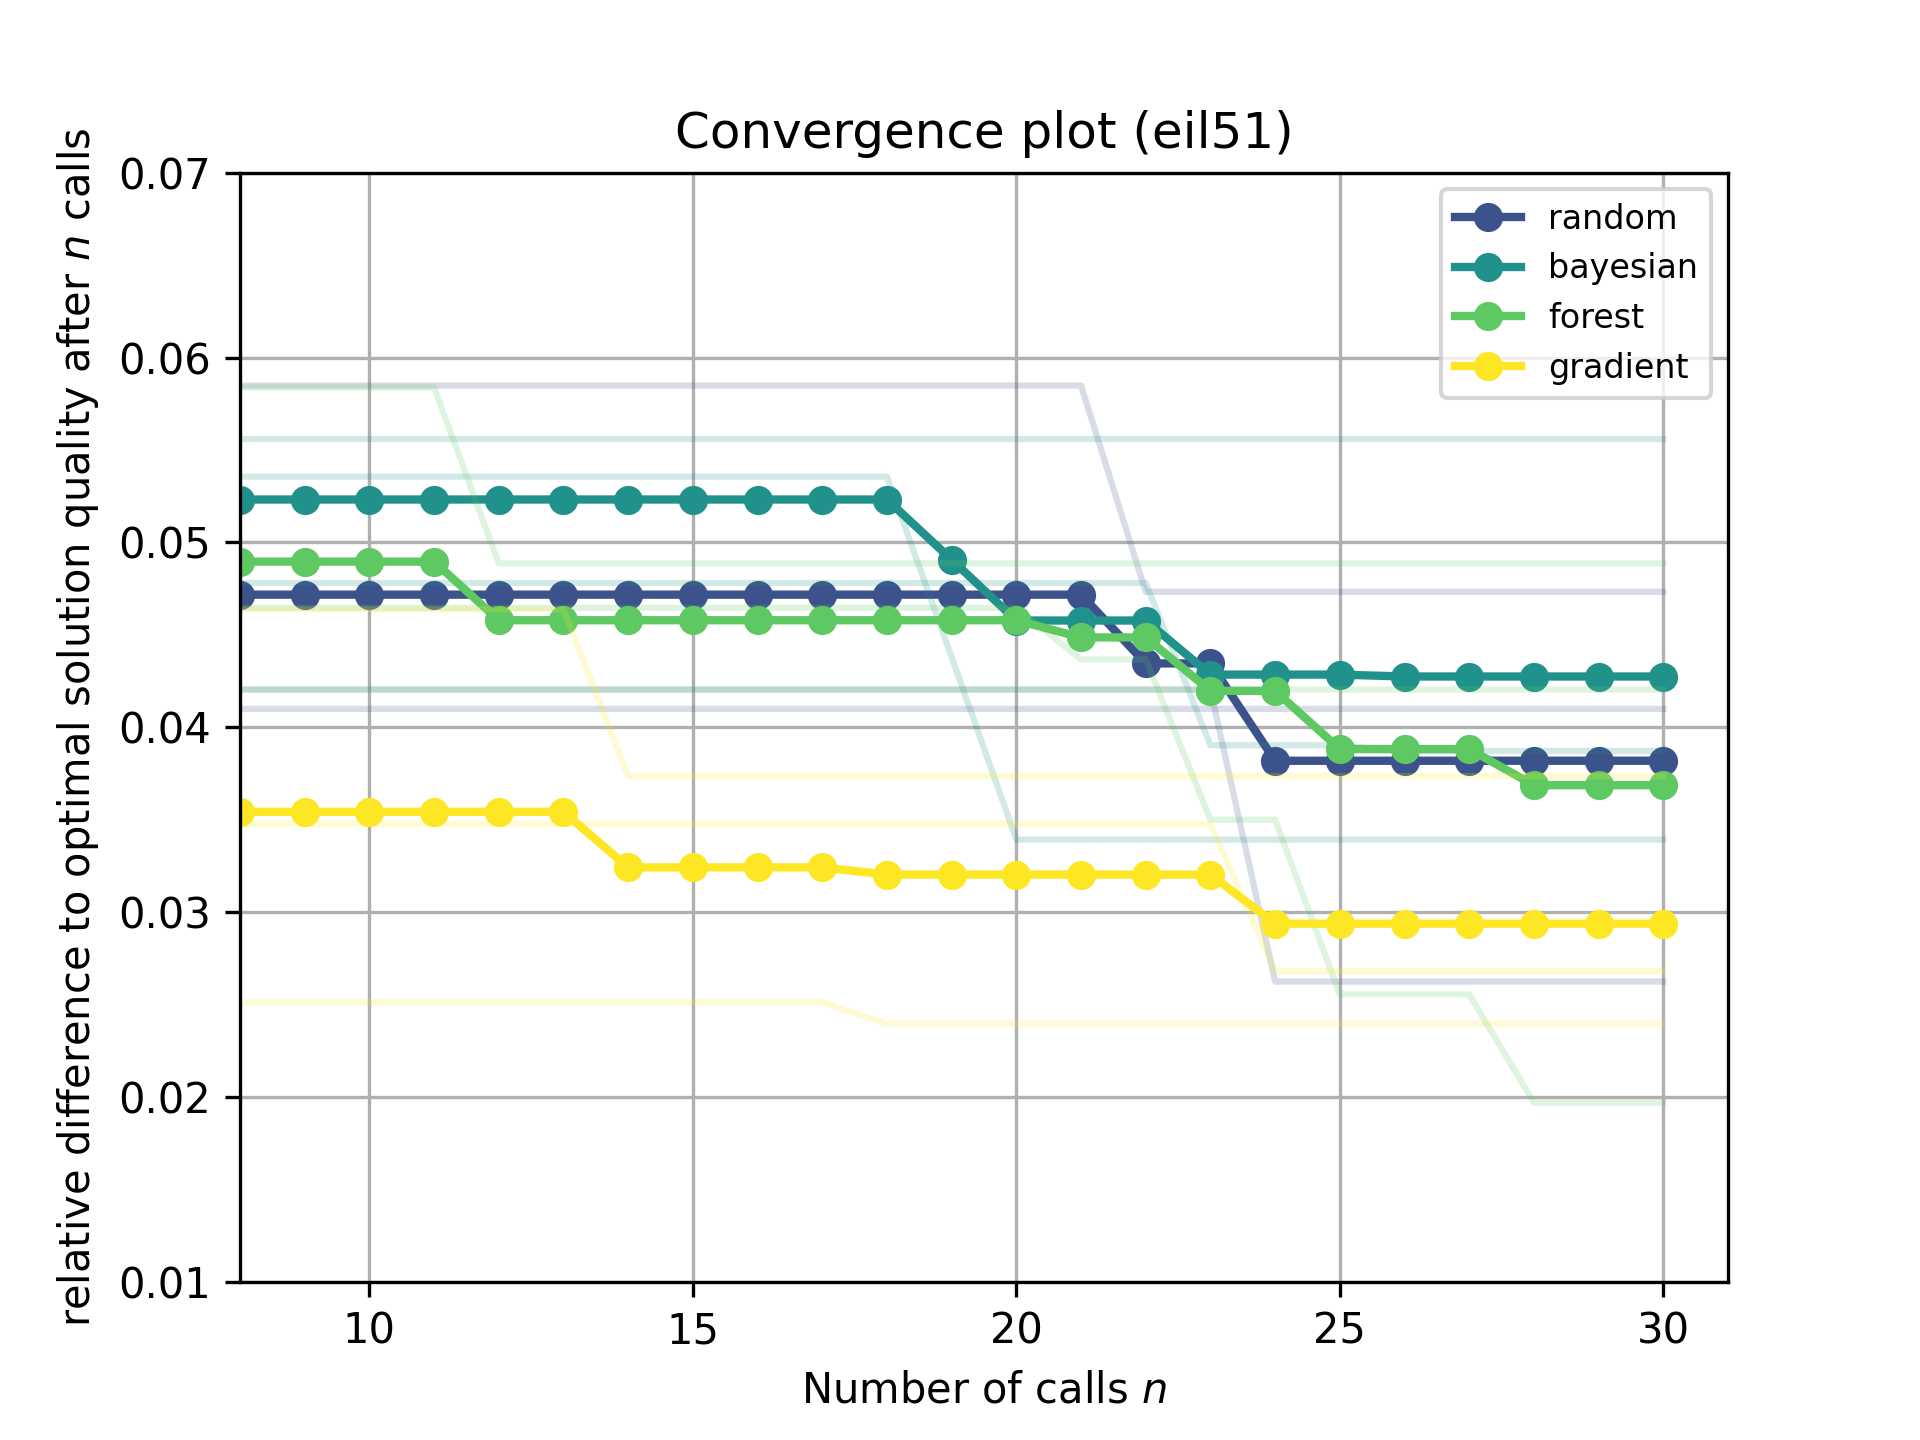
\includegraphics[width=0.75\textwidth]{results/part1/convergence_eil51.png}
	\caption[Convergence plot of \gls{tsp} instance \texttt{eil51}]{Convergence plot of \gls{tsp} instance \texttt{eil51}, comparing four different optimization algorithms.}
	\label{fig:convergence_eil51}
\end{figure}

First, the convergence plots of all five individual instances and their average are discussed. As explained in \cref{chap:an-part1}, these graphs show the minimum of the relative difference to the optimal solution $RPD$ up to each objective function call (\texttt{n\_call}). \cref{fig:convergence_eil51} shows this plot for the \texttt{eil51} \gls{tsp} instance. The bold, yellow line, which shows the average of the three \gls{gbrt} runs, indicates, that this algorithm found the best solution over the course of the 30 objective calls. Except for a single run, where \gls{et} performed admirably, achieving a 2\% difference from the optimal solution, none of the other algorithms were able to come close to the \gls{gbrt}. However, the average convergence behavior of all four algorithms seems to be very similar, with moderate improvements between objective calls 17 and 25. This behavior suggests, that the first 10 sampling calls were sufficient to obtain a decent parameter configuration for the \texttt{eil51} instance. The specific runs (light colored lines) show, that \gls{rs} and \gls{et} fluctuated the most in terms of initial solution quality and improvement over time. Although \gls{gp} produced the worst solutions out of all four algorithms, it still managed to achieve an average solution quality of almost 4\% after the full 30 \texttt{n\_calls}.

\begin{figure}[h]
	\centering
	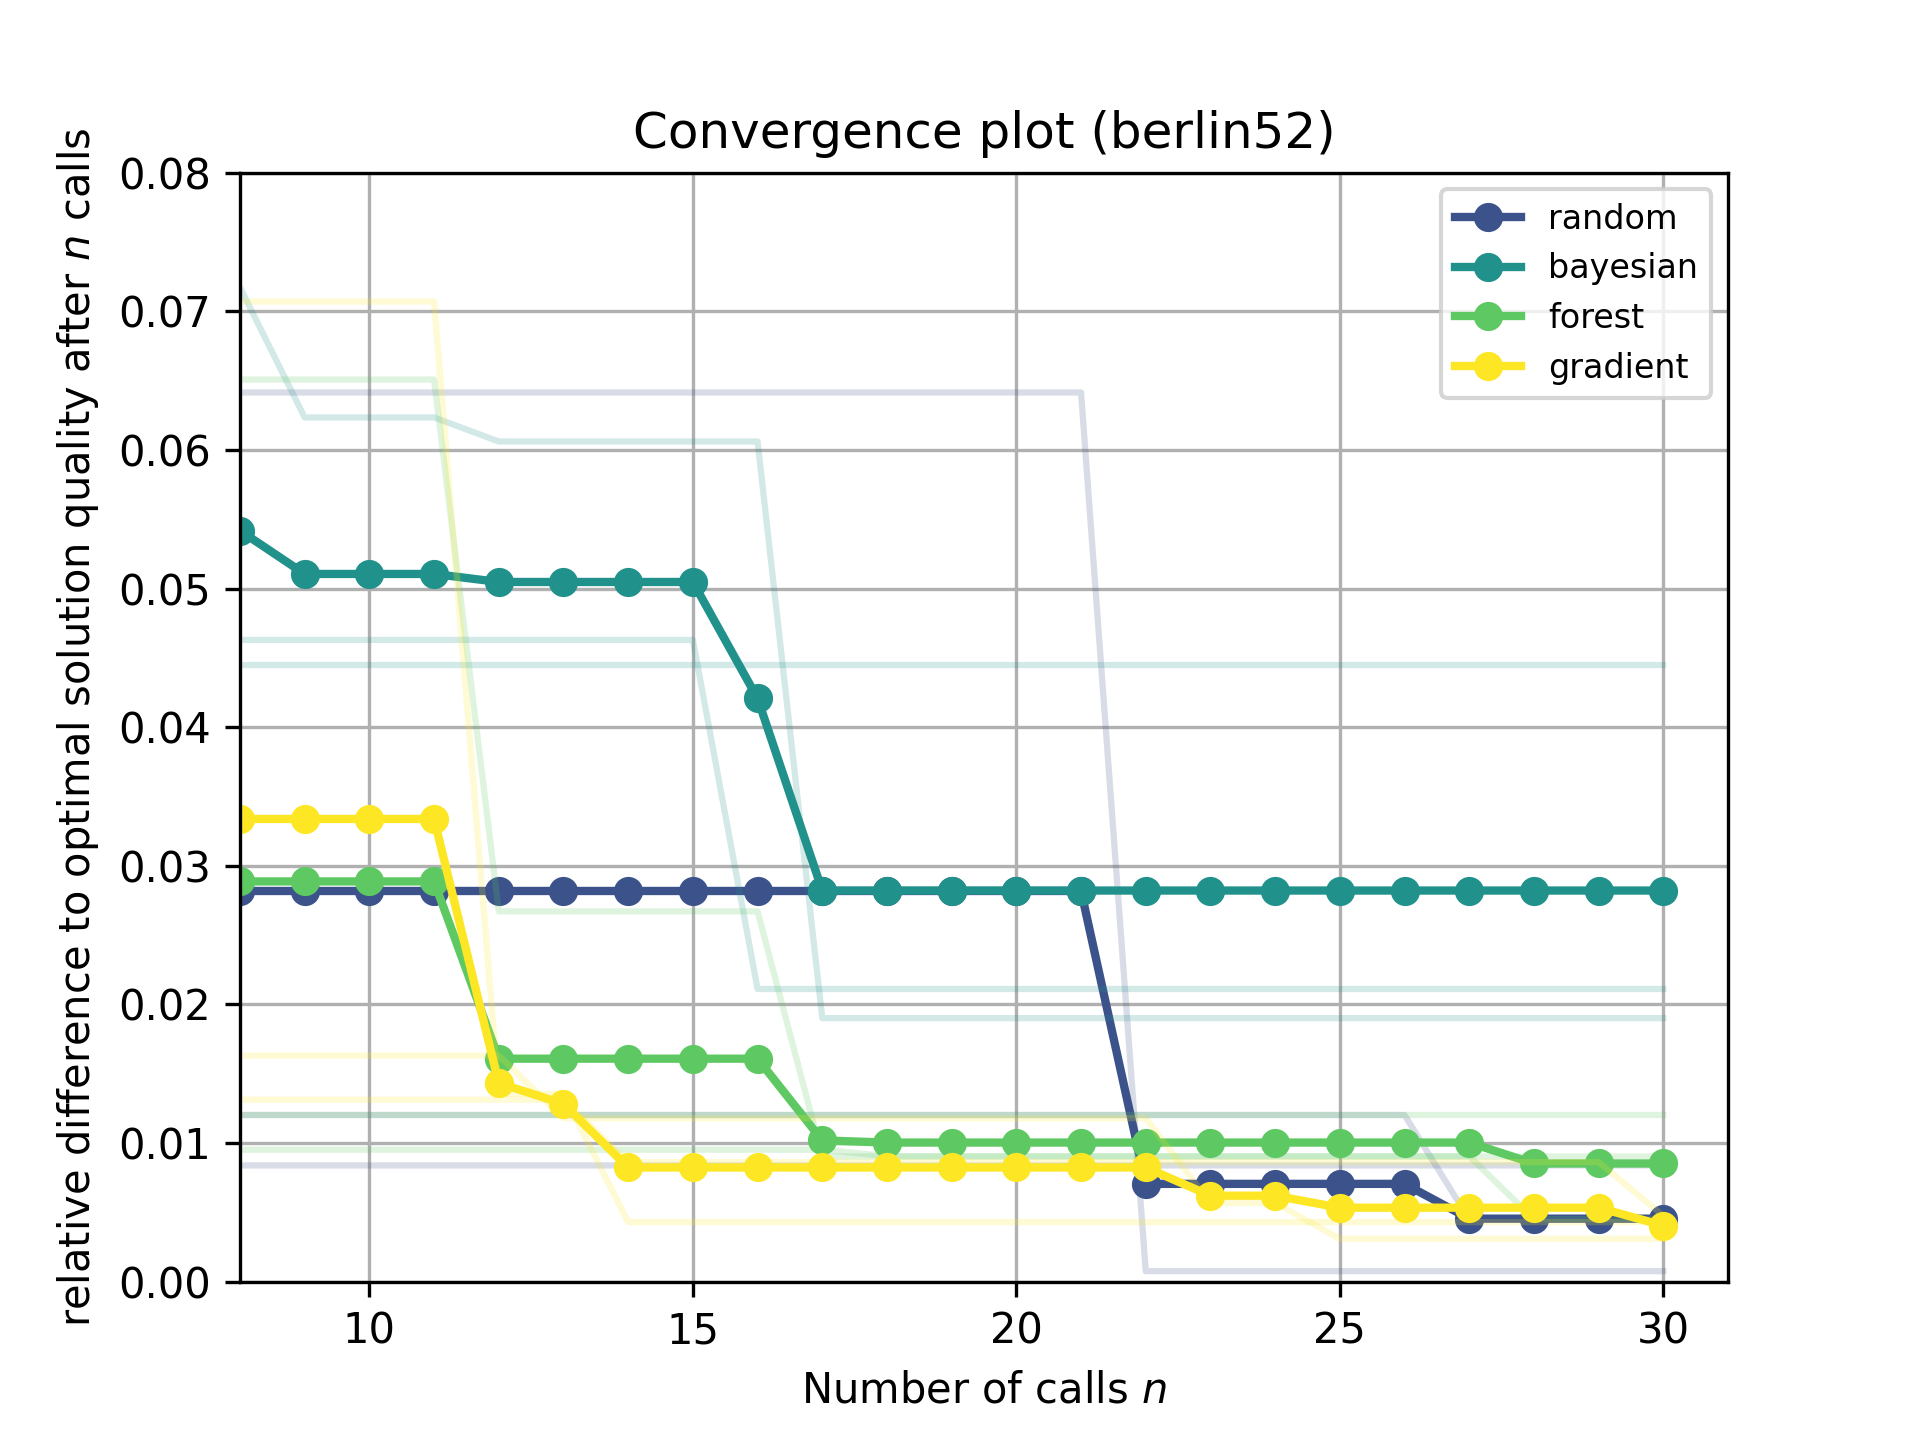
\includegraphics[width=0.75\textwidth]{results/part1/convergence_berlin52.png}
	\caption[Convergence plot of \gls{tsp} instance \texttt{berlin52}]{Convergence plot of \gls{tsp} instance \texttt{berlin52}, comparing four different optimization algorithms.}
	\label{fig:convergence_berlin52}
\end{figure}

The next instance is \texttt{berlin52}, whose convergence plot is shown in \cref{fig:convergence_berlin52}. Here, \gls{gp} continues to be the least well performing \gls{hpo} method, with an average $RPD$ of only about 3\%, with one particular run reaching as low as $4.5\%$. All other methods achieved at least 2\% lower $RPD$ values, with \gls{rs} and \gls{gbrt} having an almost identical final $RPD$ of 0.5\%. 
However, \gls{gp} was able to improve its solution by a significant 2\% over the course of seven additional objective calls, suggesting that the algorithm was quickly making use of the now utilized, underlying model.
Due to the very random nature of \gls{rs}, some other individual runs started with a very high $RPD = 6.5\%$ and then, improved very abruptly after about 21 objective calls. The convergence behavior of \gls{rf} and \gls{gbrt} is quite similar and shows, that both started with a good solution already at about 3\% for the tenth objective call, and then gradually improved up to objective call 17, analogous to \gls{gp}, but with less relative improvement. After that, only small gains in solution quality were achieved.

\begin{figure}[h]
	\centering
	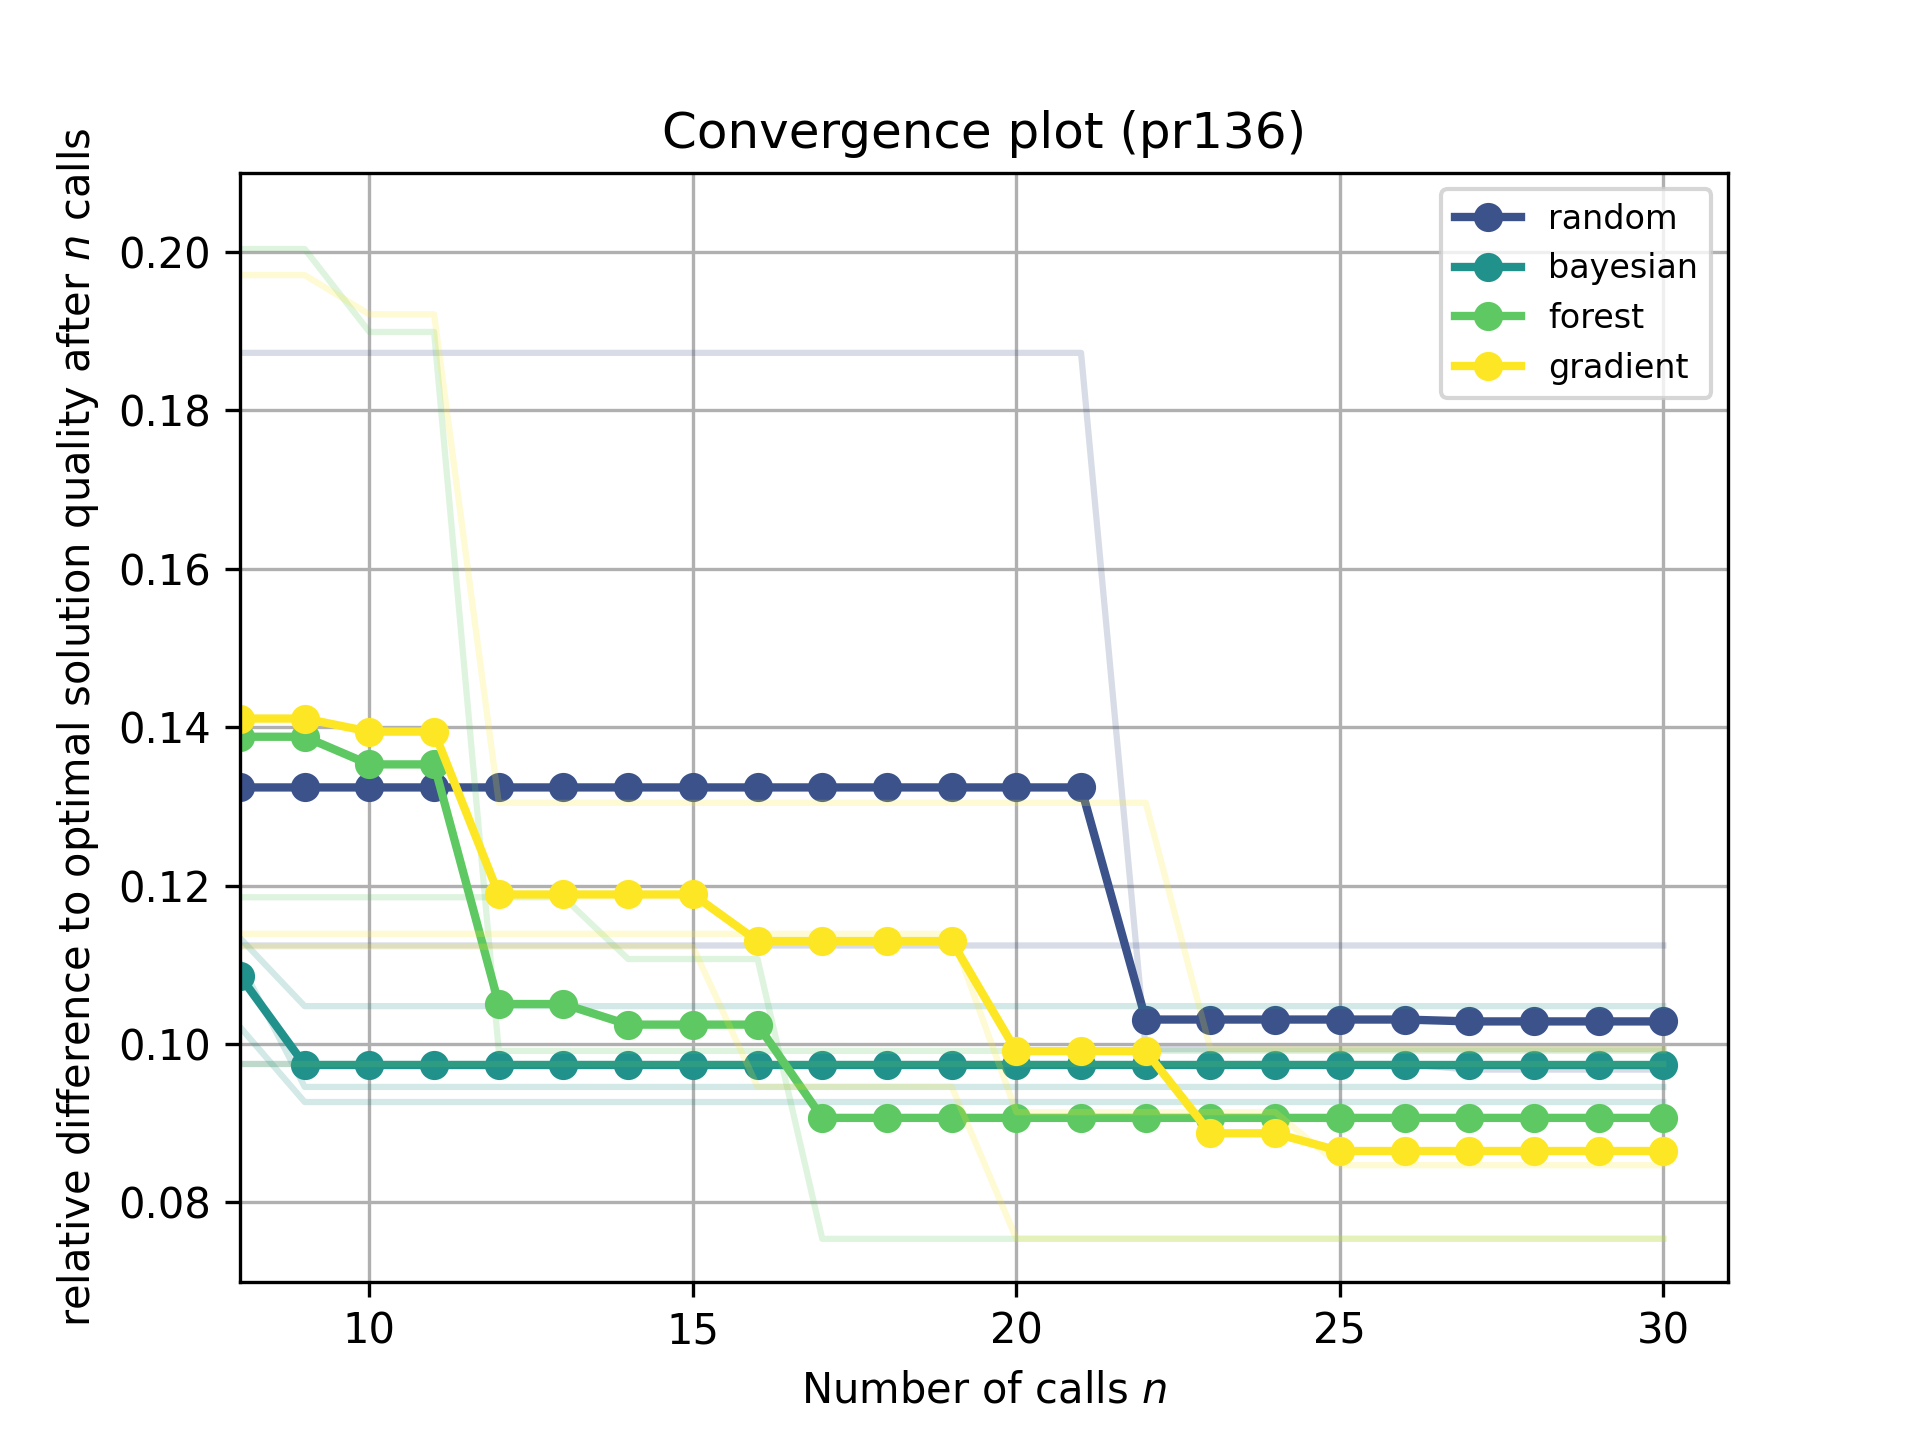
\includegraphics[width=0.75\textwidth]{results/part1/convergence_pr136.png}
	\caption[Convergence plot of \gls{tsp} instance \texttt{pr136}]{Convergence plot of \gls{tsp} instance \texttt{pr136}, comparing four different optimization algorithms.}
	\label{fig:convergence_pr136}
\end{figure}

The \texttt{pr136} \gls{tsp} instance, presented in \cref{fig:convergence_pr136}, continues the trend of \gls{gbrt} performing the best of the four optimization algorithms, albeit with a small lead of less than 0.5\% over the next best method, \gls{et}. Interestingly, \gls{gp} started with a considerably better initial sample at $RPD = 11\%$ after 10 objective calls, which gave it a head start, but also caused the algorithm to stagnate over the course of the remaining 20 calls. This might be due to the fact that Hammersley sampling was chosen only for this particular algorithm, or it could just be another random influence. \gls{et} and \gls{gbrt} gradually improved the most out of the four methods, with steep drops of around 2\% or more by the 23rd objective call. \gls{rs} rarely saw any meaningful improvement after the initial sampling, and the huge drop in average $RPD$ was due only to a single run that remained at a relatively poor value of $RPD = 18.8\%$ up until the 21st \texttt{n\_call}.

\begin{figure}[h]
	\centering
	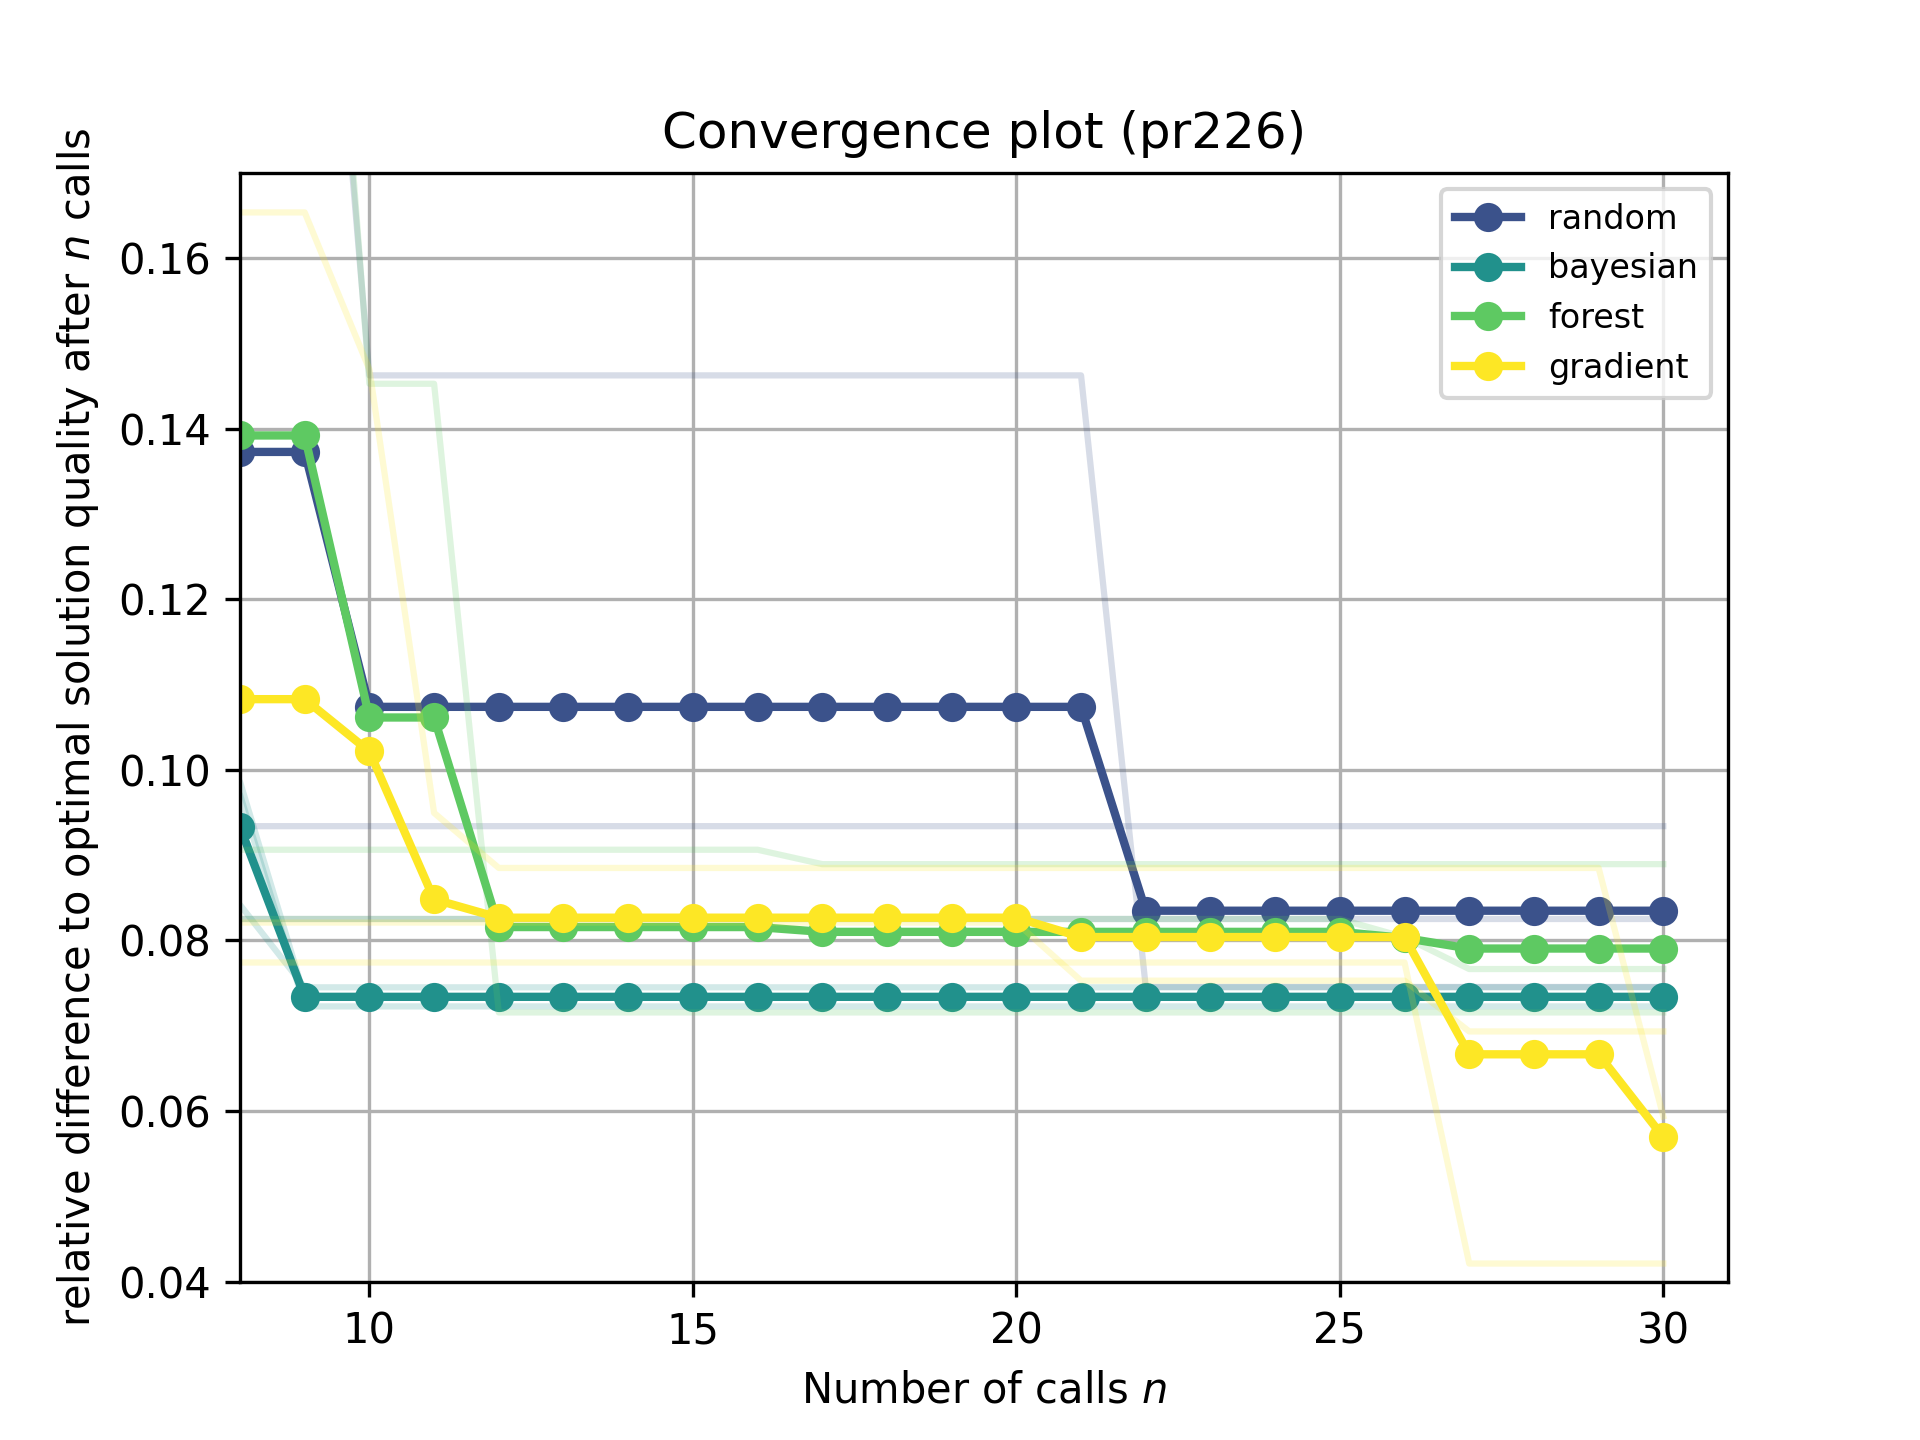
\includegraphics[width=0.75\textwidth]{results/part1/convergence_pr226.png}
	\caption[Convergence plot of \gls{tsp} instance \texttt{pr226}]{Convergence plot of \gls{tsp} instance \texttt{pr226}, comparing four different optimization algorithms.}
	\label{fig:convergence_pr226}
\end{figure}

The convergence plot in \cref{fig:convergence_pr226} for instance \texttt{pr226} again has \gls{rs} as the weakest method, with only small gains of about 2\% on objective call 22, bringing it to the average $RPD$ of the other algorithms. Some other single runs performed even worse. Contrary to the good performance of the other instances, this time \gls{et} starts its model training at 10 objective calls with a $RPD$ value almost the same as \gls{rs}, and only manages to significantly improve its parameters two \texttt{n\_calls} later. It then shows stagnant behavior at $RPD = 8\%$. Only in the last five objective calls \gls{gbrt} showed a similar convergence behavior, improving by more than 2\%, giving it the lead over \gls{gp}. This suggests that with larger instance dimensions and thus potentially more complex solutions, \gls{gbrt} benefits from more objective calls that improve the underlying model.
As with \texttt{pr136}, the initial sample of the Hammersley method gave \gls{gp} a lead in solution quality, but then stagnated after the ninth call and was unable to improve its $RPD$ value of about 7.5\%.

\begin{figure}[h]
	\centering
	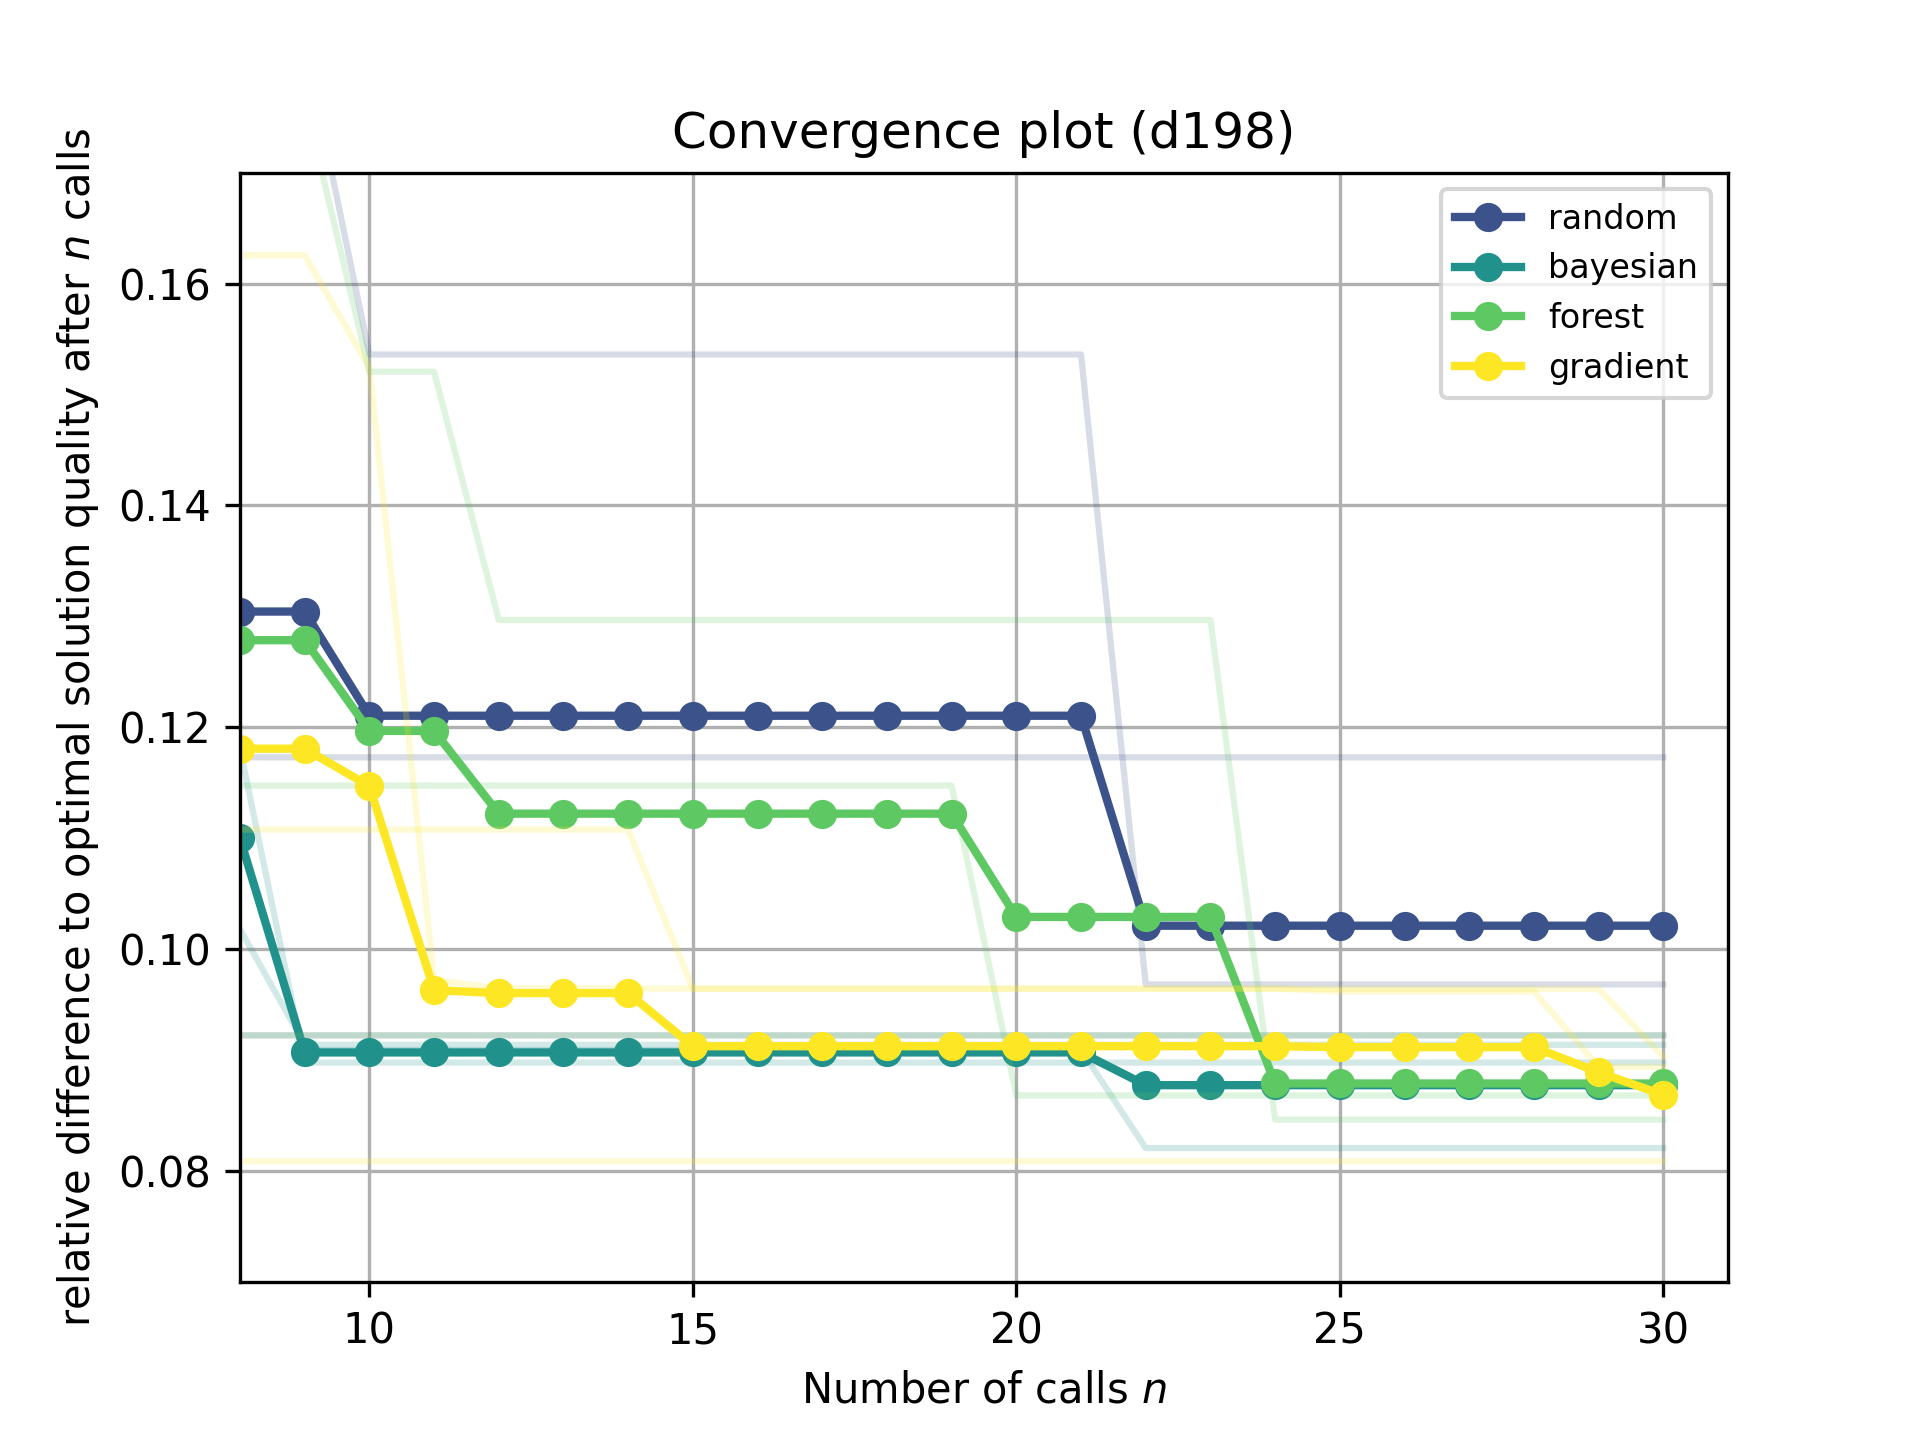
\includegraphics[width=0.75\textwidth]{results/part1/convergence_d198.png}
	\caption[Convergence plot of \gls{tsp} instance \texttt{d198}]{Convergence plot of \gls{tsp} instance \texttt{d198}, comparing four different optimization algorithms.}
	\label{fig:convergence_d198}
\end{figure}

The last \gls{tsp} instance, \texttt{d198}, confirms the observations of the previous instances, but this time all methods except \gls{rs} are within very close proximity to each other after the 24th objective call. Although \gls{gbrt} takes the lead in final relative solution quality with just under 9\%, it is not by much. Together with \gls{gp}, both methods managed to achieve considerable improvements up until the 15th objective call, after which they more or less stagnated. \gls{et} started with a similarly sub-optimal $RPD$ as \gls{rs} at objective call 10, but was able to improve steadily over the next 15 \texttt{n\_calls}. As expected at this point, \gls{rs} only managed to meaningfully improve in one run at objective call 21, still placing its final $RPD$ more than 1\% above the rest of the methods.

\begin{figure}[h]
	\centering
	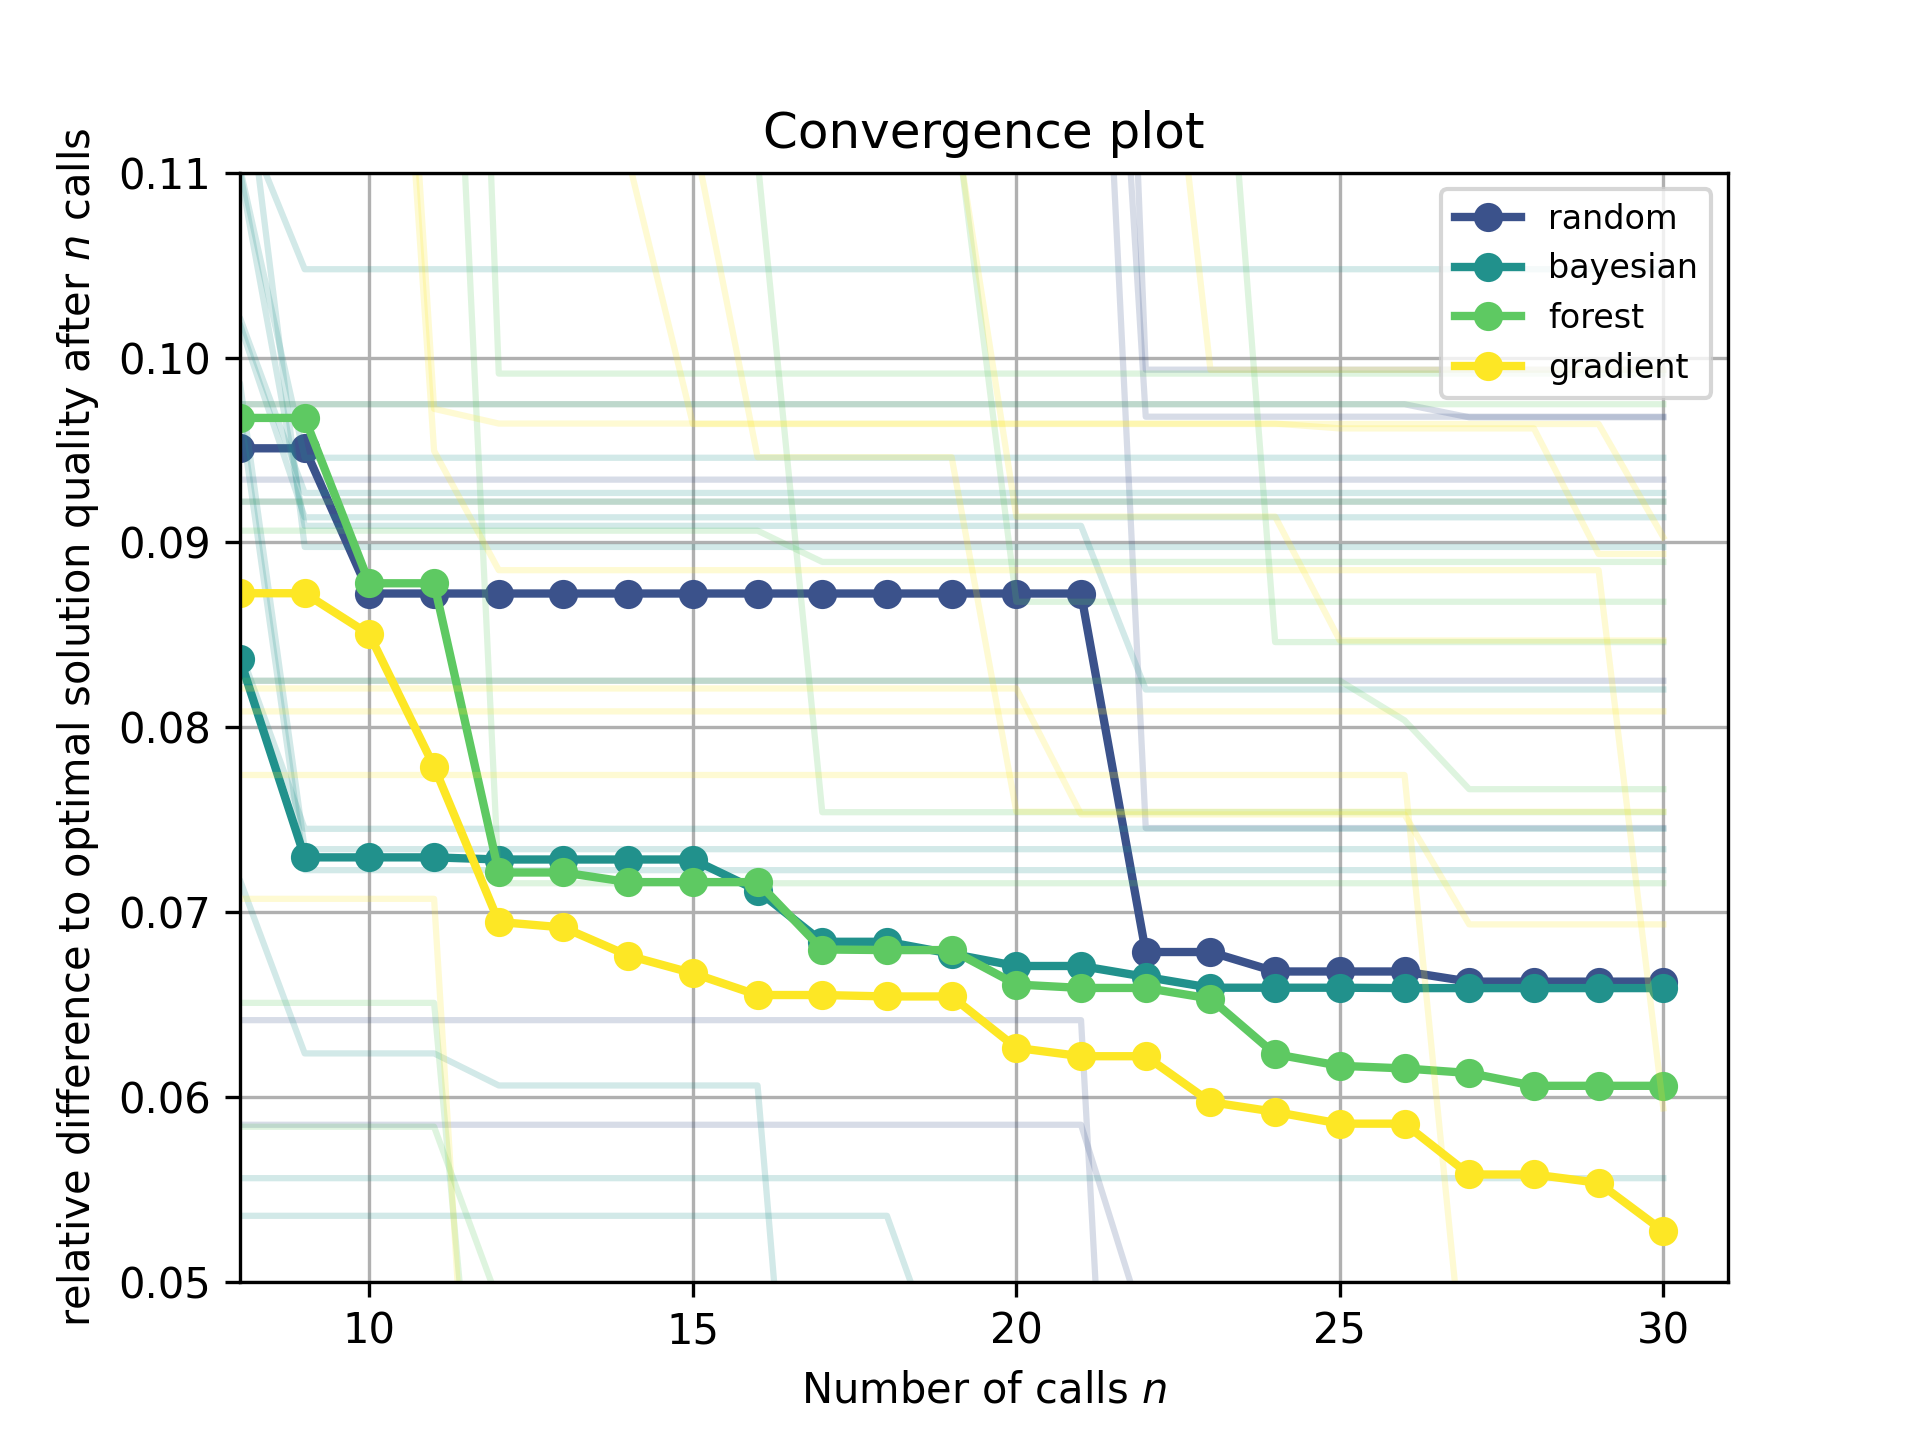
\includegraphics[width=0.75\textwidth]{results/part1/convergence_all.png}
	\caption[Convergence plot of the average over five \gls{tsp} instances]{Convergence plot of the average over five \gls{tsp} instances \texttt{eil51, berlin52, pr136, pr226, d198}, comparing four different optimization algorithms.}
	\label{fig:convergence_all}
\end{figure}

Lastly, the average convergence plot aggregates the runs of all five instances. Since \gls{gbrt} is the best performing method out of all the individual comparisons, its average convergence behavior emphasizes this by giving it a lead in final $RPD$ of about 1.5\% over the next best method, \gls{et}. Both of the show similar convergence behavior over the entire runtime, with large improvements in the first few objective calls, and small, but steady (almost linear) improvements thereafter. The behavior of \gls{gp} is not very different, and is mainly distinguished by its better initial $RPD$ value, which reinforces the proposed relationship with the Hammersley sampling method. After this initial lead, the algorithm almost stagnates, and after the 22nd objective call, it converges to the trajectory of \gls{rs}.

\begin{table}[h]
	\centering
	\caption[The \gls{auc} and $RPD_{min}$ for all optimization runs]{The \gls{auc} and minimum relative solution quality at the last objective call ($RPD_{min}$) of all optimization runs for each method and instance, and for the mean over all instances.}
	\label{tab:part1-stats}
	\begin{tabular}{c !{\vrule width 1pt} c c !{\vrule width 1pt} c  c !{\vrule width 1pt} c  c }

		~ & \multicolumn{2}{c !{\vrule width 1pt}}{eil51} &  \multicolumn{2}{c !{\vrule width 1pt}}{berlin52} &  \multicolumn{2}{c}{pr136} \\
		~ & \gls{auc} & $RPD_{min}$ & \gls{auc} & $RPD_{min}$ & \gls{auc} & $RPD_{min}$ \\ \noalign{\hrule height 1pt}
		RS & 0.830 & 0.026 & 0.347 & 0.001  & 2.266 & 0.097 \\
		GP & 0.900 & 0.034 & 0.650 & 0.019 & 1.850 & 0.093 \\ 
		ET & 0.819 & 0.020 & 0.227 & 0.005 & 1.809 & 0.075 \\ 
		GBRT & 0.601 & 0.024 & 0.159 & 0.003 & 1.948 & 0.075 \\ \noalign{\hrule height 1pt}
	\end{tabular}
	\bigskip\\
	\begin{tabular}{c !{\vrule width 1pt} c  c !{\vrule width 1pt} c  c !{\vrule width 1pt} c  c}

		~ & \multicolumn{2}{c !{\vrule width 1pt}}{pr226} & \multicolumn{2}{c !{\vrule width 1pt}}{d198} & \multicolumn{2}{c}{mean}\\
		~ & \gls{auc} & $RPD_{min}$ & \gls{auc} & $RPD_{min}$ & \gls{auc} & $RPD_{min}$ \\ \noalign{\hrule height 1pt}
		RS &  1.837 & 0.075 & 2.139 & 0.092 & 1.484 & 0.058\\ 
		GP & 1.394 & 0.072 & 1.698 & 0.082 & 1.298 & 0.060\\
		ET & 1.547 & 0.072 & 1.940 & 0.085 & 1.268 & 0.051\\ 
		GBRT & 1.497 & 0.042 & 1.745 & 0.081 & 1.190 & 0.045\\ \noalign{\hrule height 1pt}
	\end{tabular}
\end{table}

Regarding the visually observable convergence behavior of the four optimization methods, we can also look at the \glsfirst{auc} of the plots and the minimum/best relative solution quality obtained, i.e. the $RPD$ value at $\texttt{n\_call} = 30$, hereafter called $RPD_{min}$. This data is presented in \cref{tab:part1-stats} for all five instances, their mean, and is made up of all available optimizer runs.
In this context, a low \gls{auc} value would indicate that the optimization algorithm found a well-performing parameter set, and therefore a low $RPD$, in a short time, i.e., few objective calls. However, the comparatively lowest \gls{auc} does not necessarily mean that it also found the lowest $RPD_{min}$ value among all algorithms. Thus, both values are discussed for each instance to determine how fast each algorithm converged to its best solution. For the \texttt{eil51} \gls{tsp} instance, \gls{gbrt} has by far the lowest \gls{auc} of 0.601. Paired with the second best $RPD_{min} = 2.4\%$, this method continues its favorable performance from the convergence plots. With a 0.4\% improvement in $RPD_{min}$ over \gls{gbrt}, \gls{et} was the second fastest to convergence to this final solution. \gls{gp} delivered the worst performance in this instance.

The \texttt{berlin52} instance implies a similar behavior, with \gls{gbrt} leading in convergence speed via the lowest \gls{auc}. However, as discussed in the corresponding convergence plot, \gls{rs} managed to find the best solution out of the four methods, with $RPD_{min} = 0.1\%$, outperforming \gls{gbrt} by 0.2\%. Again, \gls{gp} shows the worst performance, this time with an \gls{auc} of $0.650$, almost twice as high as its direct competitor \gls{rs} with $0.347$. \gls{et} is again the second fastest converging algorithm after \gls{gbrt}, with an almost equally good $RPD_{min} = 0.5\%$.

The results for \texttt{pr136} show an equal best $RPD_{min} = 7.5\%$ for \gls{gbrt} and \gls{et}, and an almost equal \gls{auc} for \gls{gp} and \gls{et}. Therefore, in this instance, \gls{et} outperforms \gls{gbrt} as the best converging algorithm. Interestingly, even \gls{gp} achieves a better \gls{auc} of $1.850$ than \gls{gbrt}, albeit with a worse minimum relative solution quality, which is more in line with \gls{rs}.

\texttt{pr226}, the largest \gls{tsp} instance out of the five tested in this part of the experimentation discussion, continues the improvement of \gls{gp} in terms of \gls{auc}, resulting in the best value out of all four algorithms, with a solid 7\% difference compared to the next best algorithm, \gls{gbrt}, which itself, was able to achieve the best $RPD_{min}$ at 4.2\%. \gls{rs} continues to perform worse as the instance dimension increases, which could be an opposite trend for the convergence speed of \gls{gp}.

The last \gls{tsp} instance, \texttt{d198}, confirms this implication, resulting in \gls{gp} again being the best algorithm in terms of \gls{auc}, and the second best in terms of $RPD_{min}$ at 8.2\%. This suggests, that this algorithm could benefit from larger, more complex instances, perhaps even from stronger clustering, as the latter two instances were categorized. \gls{gbrt} achieved the best $RPD_{min}$ value at 8.1\% and the second best \gls{auc}, which is only 2.7\% higher than the value of \gls{gp}. In this instance, the performance of \gls{et} was comparatively underwhelming, being closer to the \gls{auc} value of \gls{rs} than to the other two methods.

Finally, the mean results confirms, that \gls{gbrt} was the algorithm that converged the fastest ($\gls{auc} = 1.19$) to the best performing parameter set ($RPD_{min} = 4.5\%$). Even in later, higher dimensional  instances, it performed at least the second best or better, implying good search consistency across the parameter space. \gls{et} obtained better solutions at an earlier time for the three smaller instances, resulting in lower averages compared to \gls{gp}, which showed the opposite trend, improving with higher problem dimension.

\begin{figure}[h]
	\centering
	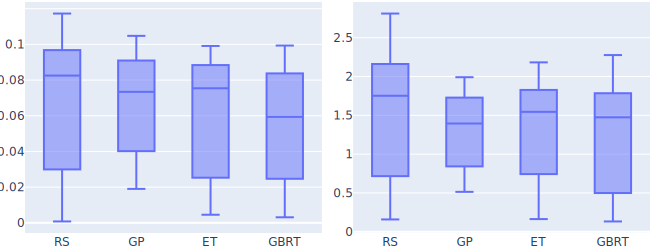
\includegraphics[width=\textwidth]{results/part1/convergence_stats_boxplot.svg}
\captionsetup[subfigure]
{skip=-8pt}
		\hfill
		\subcaptionbox{Relative difference to optimal solution quality at last the objective call ($RPD_{min}$) for all runs and instances.\label{fig:convergence_stats_boxplot_rpd_min}}[.45\linewidth]{\hfill}
		\hfill
		\subcaptionbox{\Glsfirst{auc} of solution quality convergence graph.\label{fig:convergence_stats_boxplot_auc}}[.45\linewidth]{\hfill}

	\caption[Statistical box plots illustrating convergence plots]{Statistical box plots illustrating the data of all five individual convergence plots and their individual runs.}
\label{fig:convergence_stats_boxplots}
\end{figure}

\Cref{fig:convergence_stats_boxplots} shows statistical box plots for both of the metrics from the table over all runs and not grouped by instance. This visualization is also used to evaluate the consistency across all four optimization methods, which was previously only implied by their average or best-case performance. However, this is not normalized by instance, so the absolute values and differences, as with the mean from the previous table, might not be as expressive. Nevertheless, since all four algorithms are affected by this bias, qualitative statements are still possible.

The dispersion of $RPD_{min}$ in \cref{fig:convergence_stats_boxplot_rpd_min} implies that \gls{gp} reached its solution most consistently at around its median of 7.5\%, but also never reached the same minimum as the other three algorithms. \gls{rs}, on the other hand, was the most unreliable method, with its maximum and minimum being far of from the upper and lower quartiles, respectively. It also has the highest median at about 8\%. \gls{gbrt} and \gls{et} share similarities in their \gls{iqr} and minimum/maximum values, with \gls{gbrt} having a slightly smaller dispersion. However, they differ tremendously in their median, with \gls{et} having a value almost 2\% higher than \gls{gbrt}, which means that although both their solution consistency is not ideal, \gls{gbrt} still obtained the best final solution out of all algorithms.

The box plots for the \gls{auc} (\cref{fig:convergence_stats_boxplot_auc}) show similar consistency behavior. \gls{gp} is again the most reliable algorithm when it comes to converging to its final solution, but again it cannot provide the same best-case performance (minimums) as the other three algorithms. Howeer, its median is the lowest, with \gls{gbrt} having the second lowest value, but also a significantly higher \gls{iqr} than \gls{gp}. Lastly, \gls{rs} shows the most inconsistent behavior with the highest median. 

\subsection{Statistical Tests}

To validate all of the above results, two statistical tests were also performed on the optimization data. The first test was the Kruskal–Wallis H test, explained in section \cref{chap:kruskal}, with each of the four optimization algorithms as a sample group, and separated by the five instances used. The results for each instance are shown in \cref{tab:kruskal-test}. A common significance level of 0.05 was chosen to reject the null hypothesis. The data from the table shows, that for each of the five instances, we can definitely reject the null hypothesis by looking at the $p$-values, thus suggesting that the four optimization algorithms show a significantly different convergence behavior from each other. 

\begin{table}[h]
	\centering
	\caption[Results of the Kruskal–Wallis H test for all optimization run data of the first part]{Results of the Kruskal–Wallis H test for all optimization run data of the first part, with each of the four optimization algorithms as a sample group, separated by \gls{tsp} instance.}
	\label{tab:kruskal-test}
	\begin{tabular}{l | l  l  l  l  l }
		~ & eil51 & berlin52 & pr136 & pr226 & d198 \\ \hline
		statistic & 47.893 &	46.960&	29.898	&57.998	&46.514 \\
		$p$-value & \num{2.244e-10} & \num{3.544e-10} &\num{1.450e-6} & \num{1.574e-12} & \num{4.410e-10} \\ \hline
	\end{tabular}
\end{table}
\texttt{}

A post-hoc Conover–Iman test was then performed to gain more insight into which specific pairs of optimization algorithms differ and how. As explained in \cref{chap:conover}, a one-sided test was used, resulting in two tables - one for the statistic value (\cref{tab:conover-t}) and one for the $p$-value (\cref{tab:conover-p}). Note that this table format was preferred over a symmetric matrix for each problem instance, with the columns and rows containing all five methods each. As presented here, redundant information can be excluded by directly pairing the algorithms, resulting in $\binom{4}{2} = 6$ pairs (columns) for each \gls{tsp} instance (rows). 

Starting with the $p$-value to reject the null hypothesis, we can then look at the statistic value, more specifically at the sign, to formulate the alternative hypothesis, i.e. to infer how the distribution of the convergence behavior for the algorithms differ. A positive value implies that in this particular pairwise comparison (X vs. Y), the first stated algorithm (X) has a distribution that is significantly above the others, suggesting that either the convergence speed, the solutions obtained, or both, are also worse than the second one (Y). Furthermore, in both tables the cells are marked green, whenever the $p$-value is lower than 0.05 (the significance level) and the null hypothesis can be rejected for that combination of \gls{tsp} instance and optimization method pairing.

\begin{table}[h]
	\centering
	\caption[The $p$-value of the Conover–Iman test for all optimization run data of the first part]{The $p$-value of the Conover–Iman test for all optimization run data of the first part, with each of the four optimization algorithms as a sample group, separated by \gls{tsp} instance. The cells are marked green, whenever the $p$-value is lower than the significance level of $0.05$.}
	\label{tab:conover-p}
	
	\begin{adjustbox}{width=1\textwidth}
		\begin{tabular}{ l | l  l  l  l  l  l}
			\hline
			TSP & \gls{rs} vs. \gls{gp} & \gls{rs} vs. \gls{et} & \gls{rs} vs. \gls{gbrt} & \gls{gp} vs. \gls{et} & \gls{gp} vs. \gls{gbrt} & \gls{et} vs. \gls{gbrt} \\ \hline
			eil51 & \num{0.626022837} & \num{1} & \cellcolor{green!25} \num{1,3613E-11} & \cellcolor{green!25} \num{0,045498418} &  \cellcolor{green!25} \num{9,87937E-15} &\cellcolor{green!25}  \num{1,71033E-09} \\ 
			berlin52 & \cellcolor{green!25} \num{6,31757E-10} & \num{1} & \num{0,055983678} & \cellcolor{green!25} \num{4,84375E-08} & \cellcolor{green!25} \num{5,09448E-15} & \cellcolor{green!25} \num{0,002694824} \\
			pr136 & \cellcolor{green!25} \num{4,40687E-06} &\cellcolor{green!25}  \num{1,47269E-07} & \cellcolor{green!25} \num{1,49122E-04} & \num{1} & \num{1} & \num{0,524644367} \\
			pr226 & \cellcolor{green!25} \num{1,07734E-22} & \cellcolor{green!25} \num{1,85077E-10} & \cellcolor{green!25} \num{1,83947E-11} & \cellcolor{green!25} \num{2,22893E-08} & \cellcolor{green!25} \num{2,06853E-07} & \num{1} \\ 
			d198 & \cellcolor{green!25} \num{4,0384E-15} & \cellcolor{green!25} \num{0,001090407} & \cellcolor{green!25} \num{2,6556E-07} & \cellcolor{green!25} \num{1,20061E-07} & \cellcolor{green!25}  \num{0,000563675} & \num{0,210301266}  \\ \hline
		\end{tabular}
	\end{adjustbox}
\end{table}

\begin{table}[h]
	\centering
	\caption[The $p$-value of the Conover–Iman test for all optimization run data of the first part]{The statistical value of the Conover–Iman test for all optimization run data of the first part, with each of the four optimization algorithms as a sample group, separated by \gls{tsp} instance. The cells are marked green, whenever the $p$-value is lower than the significance level of $0.05$.}
	\label{tab:conover-t}
	
	\begin{adjustbox}{width=1\textwidth}
	\begin{tabular}{ l | l  l  l  l  l  l}
		\hline
		TSP & \gls{rs} vs. \gls{gp} & \gls{rs} vs. \gls{et} & \gls{rs} vs. \gls{gbrt} & \gls{gp} vs. \gls{et} & \gls{gp} vs. \gls{gbrt} & \gls{et} vs. \gls{gbrt} \\ \hline
		eil51 & \num{-1,643854208} & \num{1,099460932} & \cellcolor{green!25} \num{8,358037955} & \cellcolor{green!25} \num{2,74331514} & \cellcolor{green!25} \num{10,00189216} & \cellcolor{green!25} \num{7,258577024} \\
		berlin52 & \cellcolor{green!25} \num{-7,486334021} & \num{-1,00169258} & \num{2,667665503} & \cellcolor{green!25} \num{6,484641441} & \cellcolor{green!25} \num{10,15399952} & \cellcolor{green!25} \num{3,669358084} \\ 
		pr136 & \cellcolor{green!25} \num{5,39986544} & \cellcolor{green!25} \num{6,222702079} & \cellcolor{green!25} \num{4,491316652} & \num{0,822836638} & \num{-0,908548788} & \num{-1,731385427} \\ 
    	pr226 & \cellcolor{green!25} \num{14,43190942} & \cellcolor{green!25} \num{7,765991183} & \cellcolor{green!25} \num{8,289835445} & \cellcolor{green!25} \num{-6,665918233} & \cellcolor{green!25} \num{-6,142073971} & \num{0,523844262} \\ 
    	d198 & \cellcolor{green!25} \num{10,20744357} & \cellcolor{green!25} \num{3,936409009} & \cellcolor{green!25} \num{6,082589453} & \cellcolor{green!25} \num{-6,271034565} & \cellcolor{green!25} \num{-4,124854122} & \num{2,146180444} \\ \hline
	\end{tabular}
	\end{adjustbox}
\end{table}

The data from both tables show, that the distribution of the \gls{gbrt} method is below all other algorithms for the \texttt{eil51} instance, although the null hypothesis in the pairing with \gls{et} was only slightly below the significance level. Furthermore, the distribution of \gls{et} was also below that of \gls{gp}, confirming the visual inference from the convergence plot. 
In the data for the \texttt{berlin52} instance, \gls{gbrt} is below \gls{gp} and \gls{et}, but interestingly, fails to reject the null hypothesis when compared to \gls{rs}, confirming the unrepresentatively good performance of this algorithm for this instance. Also, the convergence distribution of \gls{gp} is above all other three algorithms by comparison, which is also shown in \cref{fig:convergence_berlin52}.
For the next three instances, \texttt{pr136, pr226,} and \texttt{d198}, the distribution for \gls{rs} lies above all other three algorithms, verifying the underwhelming performance described in previous discussion. For the two latter instances, we can also determine that the convergence behavior of \gls{gp} is above the distribution of both \gls{et} and \gls{gbrt}.

In summary, \gls{rs} could only establish itself as having a favorable distribution only once, \gls{et} managed to have a lower convergence behavior five times, \gls{gp} could undercut in its direct pairing seven times, and \gls{gbrt} was the optimization algorithm that fell below its comparison distribution the most with 10 times. All of this confirms the favorable position of \gls{gbrt}, but also strengthens the case for \gls{gp} over \gls{et}.

\subsection{Conclusion}

As expected, \glsfirst{rs} proved to be the worst performing algorithm under these test conditions. Although each of the other three methods was able to reliably outperform its solutions, usually with fewer objective calls, it still produced satisfactory solutions that differed from the rest by only a few percent. Therefore, its aforementioned position as a \enquote{baseline} \gls{hpo} method is more than justified.

The \glsfirst{gbrt} algorithm shows the fastest convergence with the best solution quality, while providing the second most robust results. Therefore, it is used to perform the second part of the testing procedure. Another advantage, besides its good performance, is its ability to provide a trained machine learning model from which the parameter importance and other qualitative statements about its prediction can be derived.

However, the theoretical second choice is not so clear, since both \glsfirst{gp} and \glsfirst{et}, performed very well in certain instances. As suggested in some earlier discussions, \gls{et} seems to perform its best on \gls{tsp} instances with less than 100 city nodes, while \gls{gp} improves its convergence and solutions significantly on \gls{tsp} instances with dimensions above 150. Another factor may be the city placement characteristic established in \cref{chap:problem-choice}. However, confirming this possible relationship would require a different experimental setup, whereas the data from this first part would not be sufficient. Therefore, both of these algorithms should be considered as potential candidates for future tests, especially with varying problem dimensions and complexity.


\section{Part II - Choosing the Parameter Sets}
\label{chap:part2}

The second part of the experiments has been carried out using only the \glsfirst{gbrt} optimization method, but this time with double the objective calls and for all dynamic intensities applied to the smaller instances. Contrary to the previous part, there was no need to manually choose any \enquote{winner} based on the results, because the \gls{hpo} procedure provided six parameter sets and corresponding solution quality ($RPD$) for each of the 15 combinations of problem instance and dynamic (see \cref{tab:exp-setup}). From these, the best performing set with the lowest tour length $L$ was chosen and is shown in \cref{tab:best-parameters}. The parameters were explicitly chosen by this quantifiable procedure to free the further analysis from any assumptions about the the parameter aggregation process other than solution quality. While it would have been possible to average each parameter set over its six optimizer runs, or even over different dynamic intensities or problem instances, this would have introduced many unknown influences and would have allowed speculation as to which averaging method would be the most beneficial.

\begin{table}[h]
	\centering
	\caption[Best parameters from all six optimizer runs for all 15 instance combinations]{Best parameters from all six optimizer runs for all 15 combinations of \gls{tsp} instance and dynamic intensity $C$ from the second part of the experiment.}
	\label{tab:best-parameters}
	\begin{tabular}{cc | ccccccc}
		\hline
		TSP & $C$ & $\alpha$ & $\beta$ & $w_{\text{persbest}}$ & $w_{\text{persprev}}$& $w_{\text{parentbest}}$ & $\theta$ & $H$ \\ \hline
		eil51 & 0.1 & 1 & 5 & \num{0.9698012032709232} & \num{0.4970104731148196} & \num{0.9420638486560448} & \num{0.3905213054442555} & partial \\ 
		eil51 & 0.25 & 2 & 9 & \num{0.1433513703862964} & \num{0.2385297997812011} & \num{0.5412435716306161} & \num{0.3635623273846985} & full \\ 
		eil51 & 0.5 & 2 & 10 & \num{0.0587705067002678} & \num{0.959991562647809} & \num{0.4867708232028435} & \num{0.4598096104688355} & full \\ 
		berlin52 & 0.1 & 3 & 9 & \num{0.0448916769013341} & \num{0.4777787643927934} & \num{0.1957091892595615} & \num{0.2759480271198957} & partial \\ 
		berlin52 & 0.25 & 2 & 8 & \num{0.8311455041131819} & \num{0.2222104051600784} & \num{0.313274428287894} & \num{0.436036995565174} & full \\ 
		berlin52 & 0.5 & 1 & 9 & \num{0.2485751505630211} & \num{0.7739840642032905} & \num{0.9723725969016688} & \num{0.3880068267237935} & partial \\ 
		pr136 & 0.1 & 2 & 8 & \num{0.0939741840300781} & \num{0.0084471729216077} & \num{0.4693720297474018} & \num{0.3863810991570361} & partial \\ 
		pr136 & 0.25 & 2 & 10 & \num{0.038003058216178} & \num{0.6873466028167179} & \num{0.9394324689971254} & \num{0.3901585164695582} & partial \\ 
		pr136 & 0.5 & 2 & 9 & \num{0.0728348279719507} & \num{0.3253009907927114} & \num{0.6673567555329409} & \num{0.1388609048589145} & partial \\ 
		pr226 & 0.1 & 2 & 10 & \num{0.1121258043746194} & \num{0.0511444733887272} & \num{0.4363901120147211} & \num{0.1826781698597669} & partial \\ 
		pr226 & 0.25 & 2 & 9 & \num{0.4883129003158867} & \num{0.4713032045025087} & \num{0.9389513559003996} & \num{0.2397757555252823} & partial \\ 
		pr226 & 0.5 & 2 & 9 & \num{0.4276386300373169} & \num{0.1532697969130651} & \num{0.9835424877972389} & \num{0.2913396086500334} & partial \\ 
		d198 & 0.1 & 2 & 9 & \num{0.0017540098159148} & \num{0.973965162760525} & \num{0.651535106135457} & \num{0.2115440416644889} & partial \\ 
		d198 & 0.25 & 2 & 10 & \num{0.6702515127832059} & \num{0.0903011306643848} & \num{0.891733065508089} & \num{0.3858381960233191} & full \\ 
		d198 & 0.5 & 2 & 10 & \num{0.6940812792792512} & \num{0.2167360884224609} & \num{0.6662157175599704} & \num{0.2163287362343122} & partial \\ \hline
	\end{tabular}
\end{table}

These best parameter results alone would have been enough to continue with the validation in the third part, since \gls{hpo} is supposed to elevate and speed up this parameter tuning process. However, there is much information to be gained from this data set in regard to robustness, correlation between parameters and with problem descriptions, and relative parameter importance. All of this provides insight into what influences the \gls{hpo} process and, as a result, the performance of the \gls{hsppbo} metaheuristic the most.

\subsection{Robustness of Parameter Values}

First, we look at how often a certain value was chosen for a specific parameter by the \gls{hpo} and how reliable that choice is  - in short, the parameter robustness and dispersion. For that, statistical box plots were created over all 90 available optimizer runs that each contain an optimal parameter set. Each plot shows all \gls{hsppbo} parameters except the dynamic reaction type, since it only has two possible categorical values. A separate analysis for this parameter is provided afterwards instead. For each parameter's box plot the \glsfirst{iqr} can immediately be spotted as the large rectangle with a bold contour around it. A small \gls{iqr} implies low dispersion and therefore a robust parameter choice by the \gls{hpo}. The median ($Q_2$) is depicted by the separating line in the middle of the rectangle. The lower ($Q_1$) quartile line is the lower line of the rectangle and marks that 25\% of the data falls below this value, and the opposite upper ($Q_3$) quartile line shows the value of which 25\% of the data is above. Each of these two resulting regions (upper from $Q_2$ to $Q_3$ and lower $Q_2$ to $Q_1$) contain the same amount of data points. The whiskers on the top and bottom represent the upper ($Q_4$) and lower fence ($Q_0$) parameter value, respectively. Outliers are marked as dots, if their value exceeds $1.5 \times \gls{iqr}$ from the upper or lower fence or if they are $3 \times \gls{iqr}$ above $Q_3$ or below $Q_1$. All underlying statistical values can also be found in tables in \cref{chap:tables}.

\begin{figure}[h]
	\centering
	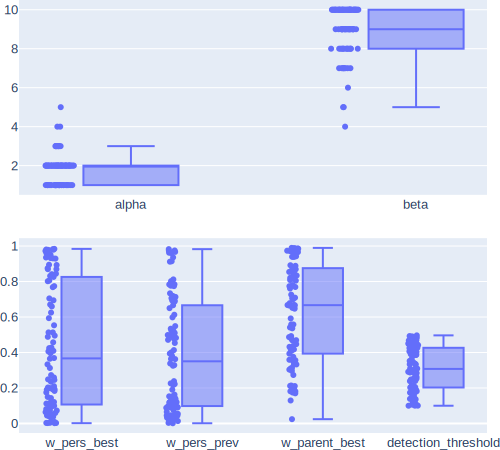
\includegraphics[width=0.85\textwidth]{results/part2/parameter_boxplot_None.svg}
	\caption[Statistical box plot of \gls{hsppbo} parameters]{Statistical box plot of all \gls{hsppbo} parameters (except $H$) over all 90 optimizer runs.}
	\label{fig:parameter_boxplot}
\end{figure}

Starting with the box plot that is not grouped over any metric, \cref{fig:parameter_boxplot} also presents, in addition to the already described information, all 90 values for each parameter as scattered dots right beside the box itself. The results for $\alpha$ imply that it is the most robust value of the six parameters, with the median falling together with the upper quartile at 2, and the minimum and lower quartile sharing their value at 1. A value of $\gls{iqr} = 1$ is remarkably low and can only be improved later on in the analysis, when looking at aggregated box plots. The surrogate model from \gls{gbrt} seemed to have no problem finding appropriate values for $\alpha$, and since a value of zero was never chosen, a floor effect can be ruled out. The $\beta$ shows a much larger spread around its median of 9 and has a very low fence of 5. However, its \gls{iqr} of 2 suggests that the \gls{hpo} process was mostly consistent in finding values for this parameter. The abrupt end of the upper quartile and maximum at 10 implies a ceiling effect (see \cref{chap:choice-param}), which was to be prevented by a large enough value range. Apparently an upper limit of 10 was not sufficient for $\beta$. But since at least 50\% of the values are below 9, this effect should not have had a significant influence on the parameter choice. 

The three weights,  $w_{\text{persbest}}, w_{\text{persprev}}$, and $w_{\text{parentbest}}$, on the other side, show considerably high dispersion. Especially the box plot for $w_{\text{persbest}}$ has an $\gls{iqr} = 0.72$, which is almost the same size as the possible value range from 0 to 1, with whiskers reaching these boundaries. Therefore, the median of 0.37 has almost no significance in choosing an optimal parameter based on means alone. This situation improves slightly when looking at the remaining two weights. Although their box plots similarly span the entire value range, their \gls{iqr} is at about half the value range ($\gls{iqr}_\text{persprev} = 0.57, \gls{iqr}_\text{parentbest} = 0.48$). Therefore, the medians of $w_{\text{persprev}}$ at 0.35 and of $w_{\text{parentbest}}$ at 0.66 can both be taken as somewhat robust. However, the fact that all three of these weights are used together in a sum makes any value suggestions an almost random one. Only the absolute parameter configuration range between 0 and 1, and a vague specification of that range for the latter two weights, can be confirmed to a degree.

The box plot for the dynamic detection threshold $\theta$ shares its y-axes with the three weights, but only has a possible value range between 0.1 and 0.5. Therefore, its \gls{iqr} is quite large at 0.22 or more than half of its range. The same dispersed behavior can be seen with its whiskers, reaching its minimum and maximum values almost precisely to the third decimal point. Without any sort of grouping applied to the data, no recommendation can be given for the detection threshold and regarding the \gls{hpo} process, this parameter could not be chosen reliably.

\begin{figure}[h]
	\centering
	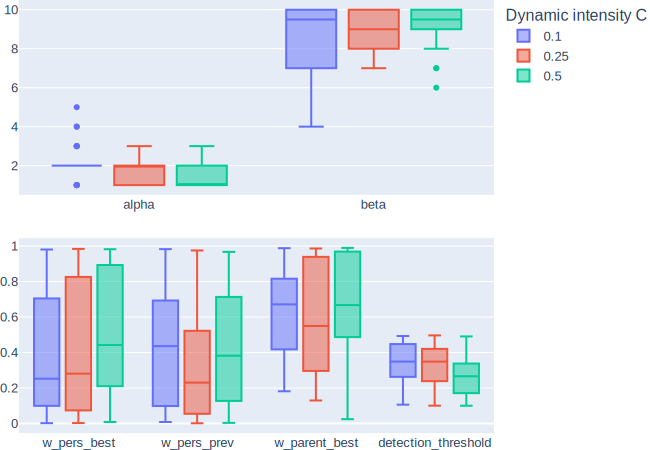
\includegraphics[width=\textwidth]{results/part2/parameter_boxplot_dynamic.svg}
	\caption[Statistical box plot of \gls{hsppbo} parameters compared by dynamic intensity]{Statistical box plot of all \gls{hsppbo} parameters (except $H$) over all 90 optimizer runs and compared by dynamic intensity $C$.}
	\label{fig:parameter_boxplot_dynamic}
\end{figure}

Continuing with the box plots shown in \cref{fig:parameter_boxplot_dynamic}, where the data points are grouped by the three tested dynamic intensities $C$, an interesting trend emerges for $\alpha$ and $\beta$. For a low dynamic intensity, meaning that very few cities swap places every $T_d = 100$ iterations, an $\alpha$ value of exactly 2 seems like the ideal choice for the \gls{hpo} process, with an \gls{iqr} of 0 and only four outliers total. $\beta$, on the other hand, shows a similar low dispersion for the highest dynamic of $C = 0.5$. With an $\gls{iqr} = 1$ and a median of 9.5, a strong heuristic influence seems to be beneficial in acquiring good solutions in highly dynamic problems. In case of $\alpha$ the other two higher dynamics introduce more spread for the value choice, but always stay in a median range between 1 and 2, with a small dispersion of 1. For $\beta$ the robustness decreases significantly with lowering dynamic intensity, reaching a high $\gls{iqr} = 3$ for $C = 0.1$.

As with the non-grouped box plots, the three weights show no sign of robust value behavior. Although small improvements can be observed for certain weights under specific dynamic intensities, e.g., $w_{\text{parentbest}}$ has a comparatively low dispersion of $\gls{iqr} = 0.4$ and reduced minimum, the spread is still far to large, in order to give any value suggestions under specific dynamic environments. The same can be said for the dynamic threshold $\theta$, where an improvement in \gls{iqr} of about 0.05, which is 12.5\% of its value range, still does not allow for a sophisticated parameter choice. The only hinted trend might be, contrary to intuition, that lower $\theta$ values benefit solving higher dynamic problem instances ($C=0.5$). However, with the median at 0.27, the upper quartile region still completely overlaps with the two other groups.

\begin{figure}[h]
	\centering
	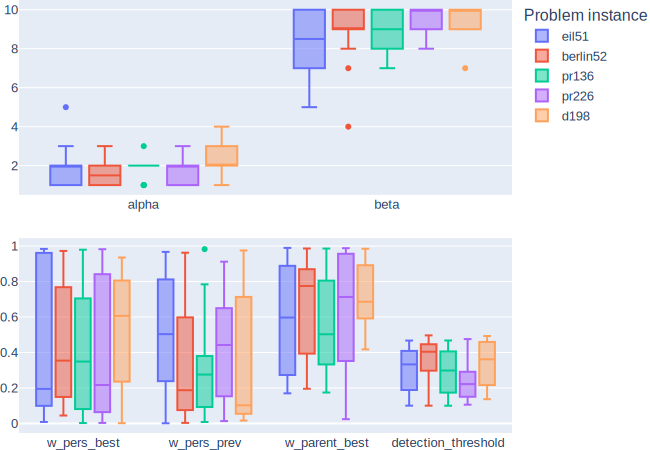
\includegraphics[width=\textwidth]{results/part2/parameter_boxplot_problem.svg}
	\caption[Statistical box plot of \gls{hsppbo} parameters compared by problem instance]{Statistical box plot of all \gls{hsppbo} parameters (except $H$) over all 90 optimizer runs and compared by problem instance.}
	\label{fig:parameter_boxplot_problem}
\end{figure}

\Cref{fig:parameter_boxplot_problem} shows the parameter box plots grouped by the \gls{tsp} problem instance they were acquired on. $\alpha$ shows low dispersion with \texttt{pr136}, an instance with medium clustered structure, and unusual high dispersion with \texttt{d198}, an instance with highly clustered areas. The other problems instances show similar results as observed before and the median for all five instances still lies between 1.5 and 2. The same conclusions can be drawn for $\beta$, where instances \texttt{berlin52, pr226}, and \texttt{d198} show a low \glspl{iqr} of 2, while the remaining two instances, especially \texttt{eil51}, show very unreliable values with medians as low as 8.5. 

The three weights, as expected from prior observations, show very dispersed distributions, with \texttt{eil51} probably being the most spread out for all values. Only some instances have an improving effect on the robustness, e.g., $w_{\text{persprev}}$ for instance \texttt{pr136} with a low $\gls{iqr} =  0.29$ and a median of 0.28, or $w_{\text{parentbest}}$ for instance \texttt{d198} with $\gls{iqr} =  0.30$ and a median of 0.69. Also, compared too the values from previous figures, $w_{\text{parentbest}}$ appears to be at lot more robust across all instances (except \texttt{pr226}), which suggests, that this value could be very dependent on the particular problem it is used for.
The detection threshold $\theta$ shows some instances, \texttt{berlin52} and \texttt{pr226}, to result in a more robust value choice with \glspl{iqr} of about 0.15, which is even better, than the aggregation by dynamic intensity shows. However, these two robust values are very different at a median of 0.40 and 0.22, respectively, which implies that the dynamic detection might be strongly influenced by the problem instance it is used on. This also shows in the data for the reaction type $H$, that in the following.
 
\begin{table}[h]
	\centering
	\caption[The distribution of the \gls{hsppbo} reaction type $H$]{The distribution of the \gls{hsppbo} reaction type $H$. Either for all parameter sets or for parameter sets grouped by dynamic intensity $C$ or problem instance, the percentages of these sets using one or the other reaction type are given.}
	\label{tab:reaction-type}
	
	\begin{tabular}{ccS[table-omit-exponent, fixed-exponent = -2, round-precision = 1]S[table-omit-exponent, fixed-exponent = -2, round-precision = 1]}
		\hline
		Comparison & Group & $H_\text{partial}$ [\si{\percent}] & $H_\text{full}$ [\si{\percent}] \\ \hline
		- & - & 0.6666666666666666 & 0.3333333333333333 \\  \hline
		\multirow{3}{*}{Dynamic Intensity} & 0.1 & 0.7666666666666667 & 0.23333333333333334 \\ 
		& 0.25 & 0.5666666666666667 & 0.43333333333333335 \\ 
		& 0.5 & 0.6666666666666666 & 0.3333333333333333 \\ \hline
		\multirow{3}{*}{\shortstack{Dynamic Intensity\\Best 50\% RPD}} & 0.1 & 0.6666666666666666 & 0.3333333333333333 \\ 
		& 0.25 & 0.5333333333333333 & 0.4666666666666667 \\ 
		& 0.5 & 0.6666666666666666 & 0.3333333333333333 \\ \hline
		\multirow{5}{*}{Problem Instance} 
		& eil51 & 0.6111111111111112 & 0.3888888888888889 \\ 
		& berlin52 & 0.7222222222222222 & 0.2777777777777778 \\ 
		& pr136 & 0.7777777777777778 & 0.2222222222222222 \\ 
		& pr226 & 0.8333333333333334 & 0.16666666666666666 \\
		& d198 & 0.3888888888888889 & 0.6111111111111112 \\  \hline
		\multirow{5}{*}{\shortstack{Problem Instance\\Best 50\% RPD}} 
		& eil51 & 0.5555555555555556 & 0.4444444444444444 \\ 
		&  berlin52 & 0.6666666666666666 & 0.3333333333333333 \\ 
		& pr136 & 0.6666666666666666 & 0.3333333333333333 \\ 
		& pr226 & 0.7777777777777778 & 0.2222222222222222 \\ 
		& d198 & 0.4444444444444444 & 0.5555555555555556 \\ \hline
	\end{tabular}
\end{table}

The parameter of the dynamic reaction mechanism $H$ was chosen to be discussed separately, because a two-valued categorical value is not effectively displayed by a box plot. Instead, \cref{tab:reaction-type} shows the distribution across the same comparison groups as used with the box plots. In addition to the two grouped versions, distributions for only the parameter sets that resulted in 50\% or better relative solution qualities ($RPD$) were added, to represent the choice for $H$ of only the best parameter sets.

It is immediately apparent, that except for some deviations, the partial reaction $H_\text{partial}$ is most often proffered by the \glsdesc{hpo}. Double the parameter sets used this method of dynamic reaction in an overall (ungrouped) comparison. For the lowest ($C=0.1$) and highest ($C=0.5)$ dynamic intensity, this preference can also be confirmed, while the medium intensity also has $H_\text{full}$ as a viable choice 43.3\% of the time. Except for a slight percetage decrease for $H_\text{partial}$ with $C=0.1$, this behavior does not change for the best 50\% of solutions.
When grouped by \gls{tsp} instance, the only problem not favoring the partial reset appears to be \texttt{d198}, where 61.1\% of parameter sets use the $H_\text{full}$ method. Contrary to this observation, the \gls{hpo} process decided to use the partial reset 83.3\% of the time for \texttt{pr226}, which is the highest bias towards any $H$ method. Looking at the best 50\% of parameter sets, \texttt{eil51} clearly deviates from any preference and has both methods almost at 50\%. The other instances also have a decrease in their bias towards $H_\text{partial}$, except for \texttt{d198}, which now seems to choose the full reset less often for its better solutions.

\subsubsection{Parameter Value Recommendations}

Based on the previous discussion of parameter robustness, their median values and possible preferences and trends regarding certain combinations of dynamic intensity and problem instance, some general recommendations for possibly well-performing parameter sets are given. These suggested value ranges might be used for a refinement of the \gls{hpo} process or could also be used as guidelines for manual parameter tuning.

Starting with the two soundest recommendations, $\alpha$ and $\beta$, which had the lowest \glspl{iqr} out of all parameter box plots. The median for $\alpha$ was almost always at 2, with boundaries rarely exceeding $[1,2]$. This was also the parameter less influenced by any change in problem description, which makes the choice of $\alpha = 2$ the most robust suggestion. $\beta$ has a median most often between $[9,10]$ and is slightly influenced by dynamic intensity and problem instances. Since some combinations had $\beta$ being chosen as low as 4, with a lower quartile value of around 7, and with the ceiling effect in mind, a value range between $[7,12]$ should result in satisfactory solutions.




\subsubsection{Influence of Problem Instances}

\begin{figure}[h]
	\centering
	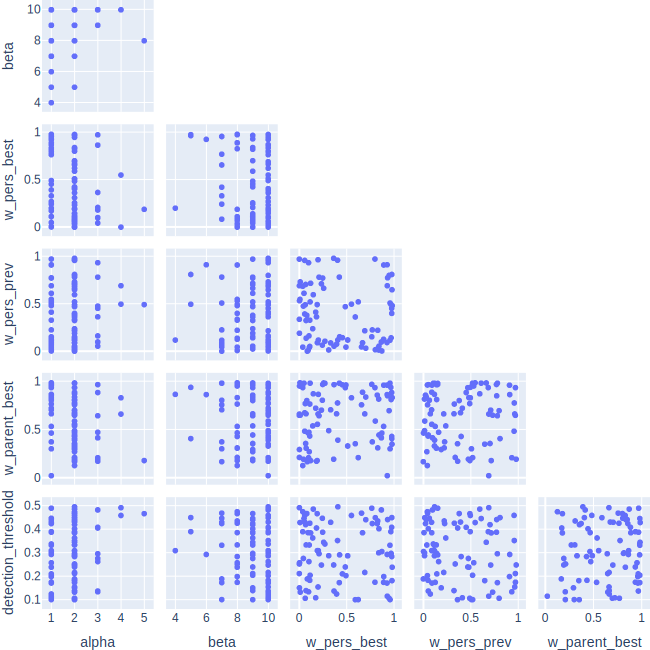
\includegraphics[width=\textwidth]{results/part2/param_scatter_matrix_None.svg}
	\caption[Scatter matrix plot of all \gls{hsppbo} parameters]{Scatter matrix plot of all \gls{hsppbo} parameters (except $H$) over all 90 optimizer runs.}
	\label{fig:parameter_scatter_matrix}
\end{figure}

\begin{figure}[h]
	\centering
	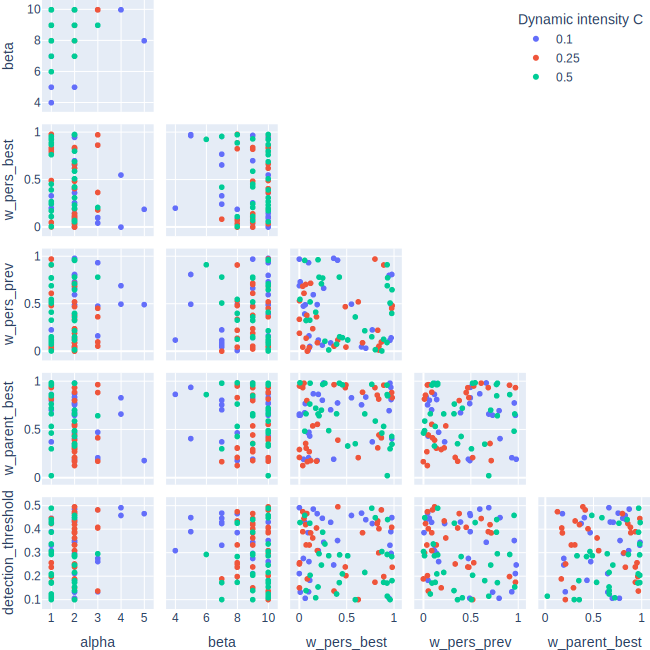
\includegraphics[width=\textwidth]{results/part2/param_scatter_matrix_dynamic.svg}
	\caption[Scatter matrix plot of all \gls{hsppbo} parameters compared by dynamic intensity]{Scatter matrix plot of all \gls{hsppbo} parameters (except $H$) over all 90 optimizer runs and compared by dynamic intensity $C$.}
	\label{fig:parameter_scatter_matrix_dynamic}
\end{figure}

\begin{figure}[h]
	\centering
	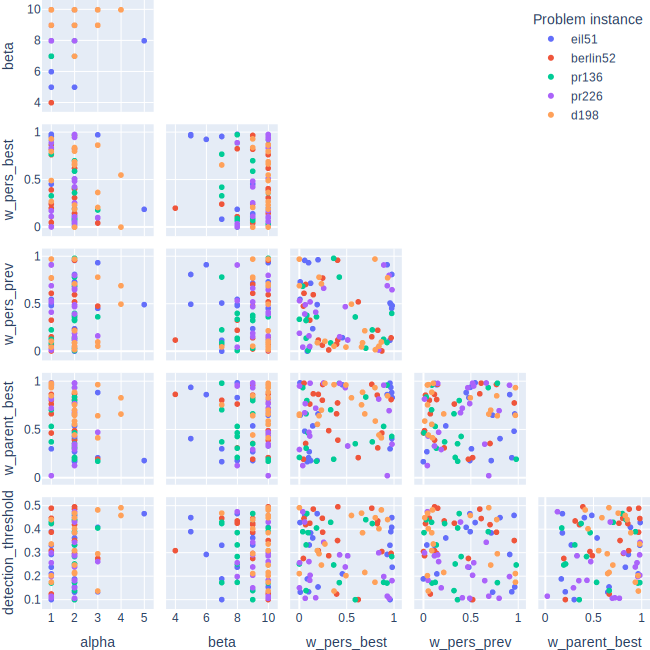
\includegraphics[width=\textwidth]{results/part2/param_scatter_matrix_problem.svg}
	\caption[Scatter matrix plot of all \gls{hsppbo} parameters compared by problem instance.]{Scatter matrix plot of all \gls{hsppbo} parameters (except $H$) over all 90 optimizer runs and compared by problem instance.}
	\label{fig:parameter_scatter_matrix_problem}
\end{figure}
\subsection{Parameter Importance}

\begin{table}[!ht]
	\centering
	\caption[Relative parameter importance over all 90 optimizer runs]{The relative parameter importance (\gls{mdi}) computed via the surrogate model over all 90 optimizer runs with the standard error. }
	\label{tab:parameter_importance}
	\begin{tabular}{cccc}
		\hline
		$\beta$ & $\alpha$ & $w_{\text{parentbest}}$ & $\theta$ \\ \hline
		  \num{0.3026887387214929} $\pm$ \num{0.0068271325972591185} & 
		  \num{0.18503797670261257} $\pm$ \num{0.005773445553779512} & 
		  \num{0.13219322556428054} $\pm$ \num{0.0048906270152243485} & 
		  \num{0.1316600435540604} $\pm$ \num{0.005210027993794393} \\ \hline
	\end{tabular}
	\bigskip\\
	\begin{tabular}{ccc}
		\hline
		$w_{\text{persprev}}$ & $w_{\text{persbest}}$ & $H$ \\ \hline
		\num{0.11494569405569222} $\pm$ \num{0.004096682063210092} & 
		\num{0.10821824956197788} $\pm$ \num{0.003648963763332609} & 
		\num{0.025256071839883553} $\pm$ \num{0.0023011990335138335} \\ \hline
	\end{tabular}

\end{table}

\begin{figure}[h]
	\centering
	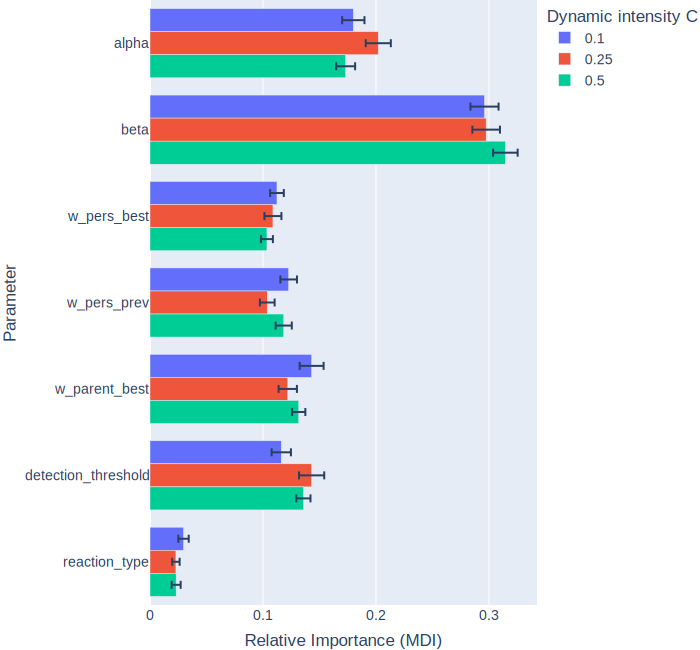
\includegraphics[width=1\textwidth]{results/part2/parameter_importance_bar_dynamic.svg}
	\caption[Bar chart of the parameter importance compared by dynamic intensity]{Bar plot of the parameter importance (\gls{mdi}) computed via the surrogate model over all 90 optimizer runs and compared by dynamic intensity $C$.}
	\label{fig:parameter_importance_bar_dynamic}
\end{figure}

\begin{figure}[h]
	\centering
	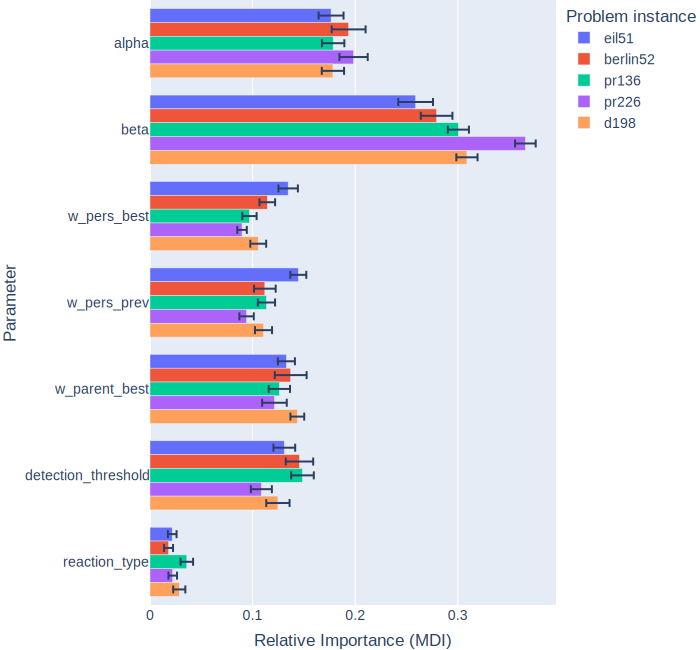
\includegraphics[width=1\textwidth]{results/part2/parameter_importance_bar_problem.svg}
	\caption[Bar plot of the parameter importance compared by problem instance]{Bar plot of the parameter importance (\gls{mdi}) computed via the surrogate model over all 90 optimizer runs and compared by problem instance.}
	\label{fig:parameter_importance_bar_problem}
\end{figure}


\begin{figure}[h]
	\centering
	\centerline{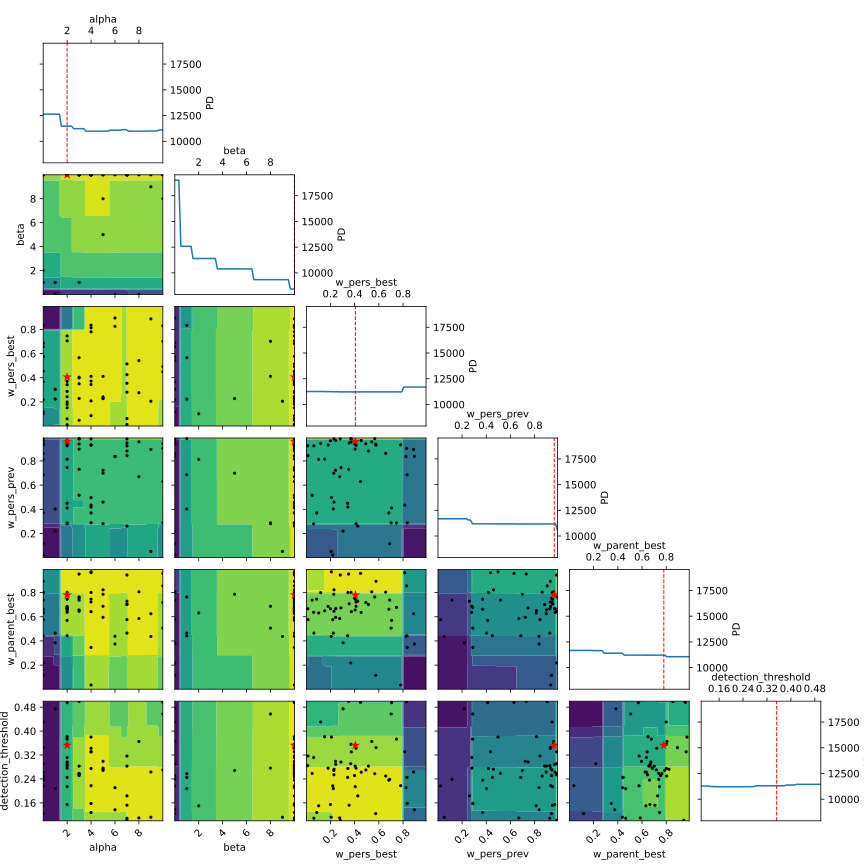
\includegraphics[width=1.2\textwidth]{results/part2/partial_dependence_berlin52_C_0.1_run_2.svg}}
	\caption[Partial dependence plot for \texttt{berlin52} and $C=0.1$]{Partial dependence plot using the surrogate model of the optimizer run with the best parameter set for problem instance \texttt{berlin52} and dynamic intensity $C=0.1$. Better (smaller) solutions are lightly colored, dark areas represent worse solution areas.}
	\label{fig:partial_dependence_berlin52_C_01}
\end{figure}

\begin{figure}[h]
	\centering
	\centerline{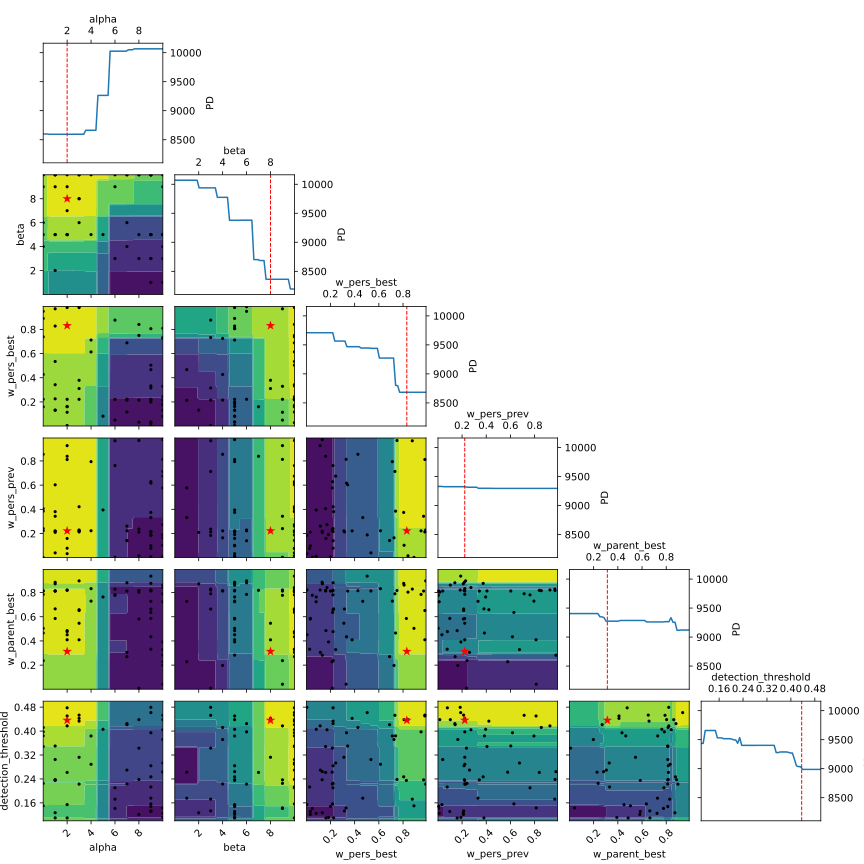
\includegraphics[width=1.2\textwidth]{results/part2/partial_dependence_berlin52_C_0.25_run_4.svg}}
	\caption[Partial dependence plot for \texttt{berlin52} and $C=0.25$]{Partial dependence plot using the surrogate model of the optimizer run with the best parameter set for problem instance \texttt{berlin52} and dynamic intensity $C=0.25$. Better (smaller) solutions are lightly colored, dark areas represent worse solution areas.}
	\label{fig:partial_dependence_berlin52_C_025}
\end{figure}

\begin{figure}[h]
	\centering
	\centerline{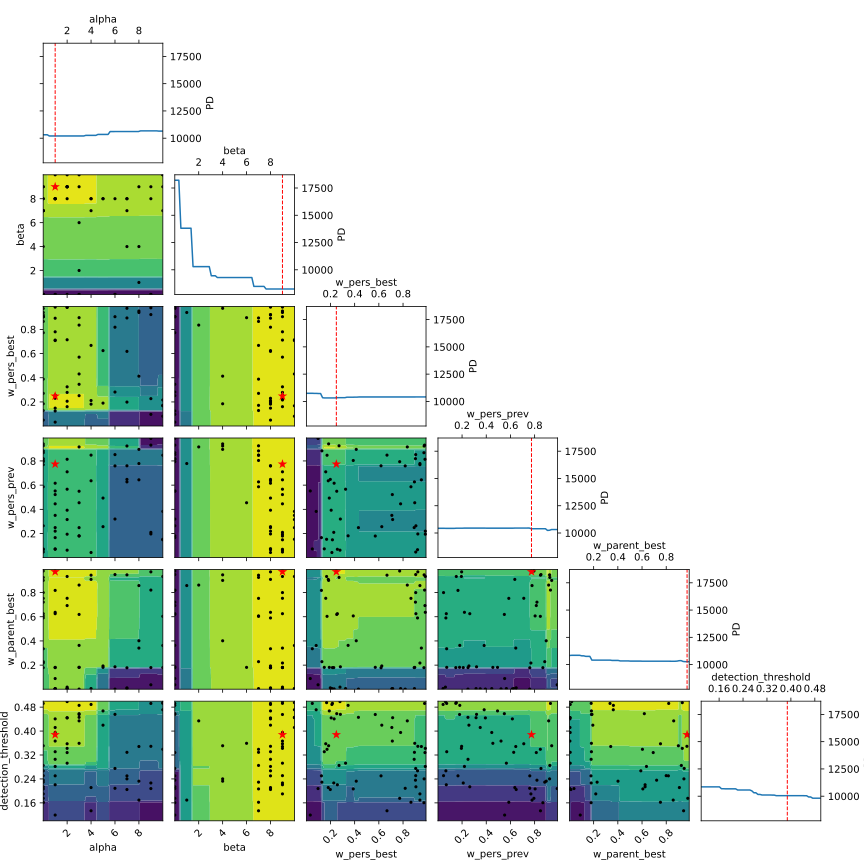
\includegraphics[width=1.2\textwidth]{results/part2/partial_dependence_berlin52_C_0.5_run_4.svg}}
	\caption[Partial dependence plot for \texttt{berlin52} and $C=0.5$]{Partial dependence plot using the surrogate model of the optimizer run with the best parameter set for problem instance \texttt{berlin52} and dynamic intensity $C=0.5$. Better (smaller) solutions are lightly colored, dark areas represent worse solution areas.}
	\label{fig:partial_dependence_berlin52_C_05}
\end{figure}

\section{Part III - Evaluating the Parameter Sets}
